\documentclass[10pt,conference]{IEEEtran}
\IEEEoverridecommandlockouts

\usepackage[utf8]{inputenc}
\usepackage[T1]{fontenc}
\usepackage{amsmath,amssymb,amsfonts}
\usepackage{algorithmic}
\usepackage{graphicx}
\usepackage{textcomp}
\usepackage{booktabs}
\usepackage{framed}
\usepackage{float}
\usepackage{xcolor}
\usepackage{footnote}
\usepackage{xfrac}
\usepackage{balance}
\usepackage{hyperref}
\usepackage{array}
\usepackage{subfigure}
\newcolumntype{L}[1]{>{\raggedright\let\newline\\\arraybackslash\hspace{0pt}}m{#1}}

\usepackage{listings}

\definecolor{mygreen}{rgb}{0,0.6,0}
\definecolor{lightgreen}{rgb}{0.6,0.9,0.6}
\definecolor{lightyellow}{rgb}{0.9,0.9,0.6}
\definecolor{lightorange}{rgb}{0.9,0.8,0.6}
\definecolor{lightred}{rgb}{0.9,0.7,0.7}
\definecolor{mygray}{rgb}{0.5,0.5,0.5}
\definecolor{lightgray}{rgb}{0.8,0.8,0.8}
\definecolor{mymauve}{rgb}{0.58,0,0.82}


\usepackage{pifont}
\newcommand{\lstbg}[3][0pt]{{\fboxsep#1\colorbox{#2}{\strut #3}}}

\lstdefinestyle{CStyle} {
    language=C,
    backgroundcolor=\color{white},   % choose the background color
    basicstyle=\ttfamily\scriptsize,        % size of fonts used for the code
    breaklines=true,                 % automatic line breaking only at whitespace
    captionpos=b,                    % sets the caption-position to bottom
    commentstyle=\color{mygray}\bfseries,    % comment style
    escapeinside={\%*}{*)},          % if you want to add LaTeX within your code
    keywordstyle=\color{blue},       % keyword style
    stringstyle=\color{mymauve},     % string literal style
    frame=single,
    numbers=left,
    stepnumber=1,
    xleftmargin=2em,
    escapeinside={/*!}{!*/},
    moredelim=**[l][\color{mygreen}]{+\ },
    moredelim=*[l][\color{red}]{-\ }
}

\lstdefinestyle{JavaStyle} {
    language=Java,
    backgroundcolor=\color{white},   % choose the background color
    basicstyle=\ttfamily\scriptsize,        % size of fonts used for the code
    breaklines=true,                 % automatic line breaking only at whitespace
    captionpos=b,                    % sets the caption-position to bottom
    commentstyle=\color{mygray}\bfseries,    % comment style
    escapeinside={\%*}{*)},          % if you want to add LaTeX within your code
    keywordstyle=\color{blue},       % keyword style
    stringstyle=\color{mymauve},     % string literal style
    frame=single,
    numbers=left,
    stepnumber=1,
    xleftmargin=2em,
    escapeinside={/*!}{!*/},
    moredelim=**[l][\color{mygreen}]{+\ },
    moredelim=*[l][\color{red}]{-\ }
}


\lstdefinestyle{PHPStyle} {
    language=PHP,
    alsolanguage=HTML,
    backgroundcolor=\color{white},   % choose the background color
    basicstyle=\ttfamily\scriptsize,        % size of fonts used for the code
    breaklines=true,                 % automatic line breaking only at whitespace
    captionpos=b,                    % sets the caption-position to bottom
    commentstyle=\color{mygray}\bfseries,    % comment style
    escapeinside={\%*}{*)},          % if you want to add LaTeX within your code
    keywordstyle=\color{blue},       % keyword style
    stringstyle=\color{mymauve},     % string literal style
    frame=single,
	numbers=left,
    stepnumber=1,
	xleftmargin=2em,
    escapeinside={/*!}{!*/},
    moredelim=**[l][\color{mygreen}]{+\ },
    moredelim=*[l][\color{red}]{-\ }
}


\newcounter{lstannotation}
\setcounter{lstannotation}{0}
\renewcommand{\thelstannotation}{\ding{\number\numexpr181+\arabic{lstannotation}}}
\newcommand{\annotation}[1]{\refstepcounter{lstannotation}\label{#1}\thelstannotation}


%
% Add comments in the text
%
\newboolean{showcomments}
\setboolean{showcomments}{true}
%\setboolean{showcomments}{false}

\ifthenelse{\boolean{showcomments}}
  {\newcommand{\nb}[3]{
  {\color{#2}\small\fbox{\bfseries\sffamily\scriptsize#1}}
  {\color{#2}\sffamily\small$\triangleright~$\textit{\small #3}$~\triangleleft$}
  }
  }
  {\newcommand{\nb}[3]{}
  }

\newcommand\Sof[1]{\nb{Sofia}{red}{#1}}
\newcommand\Luis[1]{\nb{Luis}{mygreen}{#1}}
\newcommand\Rui[1]{\nb{Rui}{blue}{#1}}

\makeatletter
\newcommand\footnoteref[1]{\protected@xdef\@thefnmark{\ref{#1}}\@footnotemark}
\makeatother


\begin{document}

% \title{Fixing Vulnerabilities Hinders Maintainability}
\title{\Sof{TBA - New Titles in the comments}}
%\title{Coding practices are important to produce secure software: Teach them to your students and developers!}
%\title{The reason why you should be applying coding practices: safer software.}
%\title{What is the impact of security patches in software evolution?}
%\title{Hey, developers! You should pay more attention to your patches.}

\author{
    Anonymou(s) Author(s)

%     \IEEEauthorblockN{1\textsuperscript{st} Given Name Surname}
% \IEEEauthorblockA{\textit{dept. name of organization (of Aff.)} \\
% \textit{name of organization (of Aff.)}\\
% City, Country \\
% email address}
% \and
% \IEEEauthorblockN{2\textsuperscript{nd} Given Name Surname}
% \IEEEauthorblockA{\textit{dept. name of organization (of Aff.)} \\
% \textit{name of organization (of Aff.)}\\
% City, Country \\
% email address}
% \and
% \IEEEauthorblockN{3\textsuperscript{rd} Given Name Surname}
% \IEEEauthorblockA{\textit{dept. name of organization (of Aff.)} \\
% \textit{name of organization (of Aff.)}\\
% City, Country \\
% email address}
}

\maketitle

\begin{abstract}
Security is a requirement of utmost importance to produce software with 
high quality. However, there is still a considerable amount of 
vulnerabilities being discovered and fixed, almost weekly. We suspect 
that when developers address these vulnerabilities on their codebases, 
they actually affect the maintainability of software, potentially 
introducing other vulnerabilities. This paper evaluates the impact of 
patches to improve security on the maintainability of open-source software. 
Maintainability is measured based on the Better Code Hub’s model of 10 
guidelines using a dataset including 1335 security commits.
Results show that fixing software vulnerabilities may hinder the maintainability of 
open-source software. This is particularly the case for patches that 
address Improper Input Validation (CWE-20), Information 
Exposure (CWE-200), Improper Restriction of Operations within the Bounds of a 
Memory Buffer (CWE-119), Missing Release of Memory after Effective Lifetime
(CWE-401) and Path Traversal (CWE-22). We conclude that changes to code bases to patch 
vulnerabilities need to be performed with extra care and that security-related 
code evolution should be subject in computer curricula.
\end{abstract}

\begin{IEEEkeywords}
Security, Software Maintenance, Open-Source Software
\end{IEEEkeywords}

\section{Introduction}
%
Software quality is important because it is ultimately related to the overall
cost of developing, extending and maintaining software applications~\cite{slaughter1998evaluating}. 
Software quality characteristics include, but are not limited to functional correctness,
reliability, usability, maintainability, and security. Security is an 
important non-functional requirement during the development of software systems. 
However, there is still a considerable amount of vulnerabilities being
discovered, and fixed, almost weekly as disclosed by the Zero Day Initiative
website\footnote{Zero Day Initiative website available at
\url{https://www.zerodayinitiative.com/advisories/published/} (Accessed on \today{})}.
These vulnerabilities are gateways for attackers to penetrate systems and 
exploit their resources. As an example, at the beginning of $2020$, academics published a 
new execution attack (CacheOut) capable of leaking data from Intel CPUs across many 
security boundaries~\cite{cacheOut} $-$ a processor bug that the company attempted to 
address in previous generations and that makes every user using a CPU released before Q$4$ $2018$ vulnerable. Although not a software bug, software can mitigate this type of issues
at the cost of features and/or performance.
%

In $2011$, the International Organization for Standardization (ISO) issued an
update for software product quality ISO/IEC 25010 considering
\emph{Security} as one of the main software product quality characteristics~\cite{iso:2011}. 
However, many developers still lack the knowledge about best practices to deliver secure and high-quality software~\cite{Pothamsetty:2005:SEL:1107622.1107635, 8077802}.
Unmaintainable code is hard to test, analyze and re-use, and thus more difficult
to find vulnerabilities and defects. Therefore, writing maintainable code
supports the production of more reliable software preventing the introduction of 
faults/vulnerabilities in the code bases. ISO describes software 
maintainability as ``the degree of effectiveness and
efficiency with which a software product or system can be modified to improve
it, correct it or adapt it to changes in environment, and in requirements'' on
software quality ISO/IEC 25010~\cite{iso:2011}. Novel tools have been built to 
detect automatically software vulnerabilities (e.g., FindBugs, Infer and more). 
Despite these efforts, improving software security is not a trivial task and requires 
implementing patches that might affect software maintainability. 
Our suspiciousness is that some of the these patches may have a negative 
impact on the software maintainability and, possibly, even be the cause of the 
introduction of new vulnerabilities $-$ harming software reliability. Therefore, 
in this paper, we present an empirical study on the impact of patches of 
vulnerabilities on software maintenance across open-source software.
%
% Software maintainability can also be defined as 
% the property of software that reveals how easily the software system can be 
% maintained~\cite{IEEEComputerSociety:2014:GSE:2616205} or recover after a failure. 
% Hedegus et al.
% ($2018$)~\cite{HEGEDUS2018313}, analyzed the difference of maintainability between
% groups of refactored elements and non-refactored and conclude that the source
% code elements subjected to refactorings had significantly lower maintainability
% than the elements not modified.
% There is still little information about the impact of patching vulnerabilities
% in open-source software maintainability. \textit{Are developers affecting software
% maintainability when trying to improve software security?}, it is what we want to
% investigate.
%


As ISO does not provide any specific guidelines/formulas to calculate 
maintainability, we resort to Software Improvement Group (SIG)'s web-based source 
code analysis service Better Code Hub (BCH) to compute the software compliance 
with a set of $10$ guidelines/metrics to produce quality software 
based in ISO/IEC $25010$~\cite{Visser:2016:OREILLY}. The code metrics used by BCH 
were empirically validated in previous work~\cite{Bijlsma:2012:FIR:2317098.2317124, 8530041, cruz2019energyoriented}. 
There are other well-known standards and models that have been proposed
to increase software security: Common Criteria~\cite{common:2009} which received
negative criticism regarding the costs associated and poor technical evaluation;
the OWASP Application Security Verification Criteria~\cite{oswap:2009} which is
focused only on web applications, and a model proposed by Xu et al. ($2013$)
~\cite{6616351} for rating software security (arguably, it was one of the
first steps taken by SIG to introduce security on their maintainability model). 
%
We use BCH's toolset to provide an assessment of maintainability in 
software mainly due to the broad number of metrics used.

From a methodological 
perspective, we leveraged a dataset of $1335$ security patches collected from open-source 
software. We calculate software maintainability before and after the patch to measure its 
impact. This empirical study presents evidence that changes 
applied in the code bases to patch vulnerabilities affect code maintainability. Especially, for patches that address \emph{Improper Input Validation} (CWE-20), \emph{Information 
Exposure} (CWE-200), \emph{Improper Restriction of Operations within the Bounds of a 
Memory Buffer} (CWE-119), \emph{Missing Release of Memory after Effective Lifetime} 
(CWE-401) and \emph{Path Traversal} (CWE-22). This is important work
because there is still little information about the impact of security patches on the software
maintainability. With this study, 
we intend to highlight the need for tools to predict the impact of patches on 
maintainability~\cite{4724577}, documentation to help developers adopt security 
best practices~\cite{6311252, 7927935, MESQUIDA201519} and the importance of integrating
security-related code evolution in computer curricula.
%
%BCH compiles the ISO/IEC 25010 into a set of $10$ guidelines that are the
%base of BCH's evaluation. Two examples are the \emph{Write Simple Units of Code}
%based on the McCabe Complexity~\cite{1702388} and \emph{Keep your code base Small}
%based on the idea that smaller code bases are easier to maintain and less prone to defects~\cite{Visser:2016:OREILLY}.
%

The main contributions of the present work are:
%
\begin{itemize}
	\item An empirical study on the impact of security changes on software
	maintainability and what patterns need more attention.
	\item A replication package with all scripts and data created to perform the
	empirical evaluation, for reproducibility. Available online:
  \url{https://figshare.com/s/4861207064900dfb3372}.
\end{itemize}
%
This paper is structured as follows: section~\ref{sec:motivation} introduces an
example of a security refactoring of a known vulnerability found in the
protocol implementation of OpenSSL\footnote{\label{openssl}OpenSSL is a toolkit that
contains open-source implementations of the SSL and TLS cryptographic
protocols. Repository available at \url{https://github.com/openssl/openssl}
(Accessed on \today{})}; section~\ref{sec:methodology} describes the
methodology used to answer the research questions; section~\ref{sec:results}
presents the results and section~\ref{sec:discussion} discusses their
implications; section~\ref{sec:threats} enumerates the threats to the validity of
this study; section~\ref{sec:rw} describes the different work and existing
literature in the field of study; and, finally, section~\ref{sec:conclusions}
concludes the main findings and elaborates on future work.
%
\section{Motivation and Research Questions}\label{sec:motivation}
%
Due to time-to-market pressure and the lack of security expertise~\cite{8077802}, code-related
security flaws are generally detected \textit{after the fact}, i.e., when
hackers exploit them. It turns out that fixing these issues is as simple as
modifying the software code base. However, these patches may have a
negative impact on software maintenance --- e.g., developers might follow the
quickest solution to fix the problem and not necessarily the most elegant and
performant one. Thus, we want to understand how security patches impact
the maintainability of software. 

%%%%% NEEDS REVIEW
\Sof{As an example, consider the patch of the TLS state-machine protocol implementation in 
OpenSSL\footnoteref{openssl} to address a vulnerability where an attacker could cause a Denial-of-Service
(DoS) attack by crafting TLS messages to trigger memory allocations
corresponding to large length values. This vulnerability is listed at the Common
Vulnerabilities and Exposures dictionary as CVE-$2016$-$6307$~\footnote{CVE-$2016$-$6307$
details available at \url{http://cve.mitre.org/cgi-bin/cvename.cgi?name=CVE-2016-6307}
(Accessed on \today{})}. It is amongst the vulnerabilities studied in our
research. The snippet, in Listing~\ref{lst:vuln}, presents the changes performed on the
\emph{ssl/statem/statem.c} file\footnote{CVE-$2016$-$6307$ fix available  at
\url{https://github.com/openssl/openssl/commit/c1ef7c971d0bbf117c3c80f65b5875e2e7b024b1}
(Accessed on \today{})} by the OpenSSL developers to patch the vulnerability. Every SSL/TLS connection begins with a handshake which is responsible by the
negotiation between the two parties. The problem in
CVE-$2016$-$6307$ is that due to a flaw in the logic of version $1.1.0$,
the memory for a message is allocated too early, prior to the excessive
message length check which can lead to a Denial of Service through memory
exhaustion if an attacker triggers up a certain message length to be allocated to service a
connection. In this case, there is only a security impact if the application does not call  \texttt{SSL\_free()} in a timely manner in the
event that the connection fails;
or, the application is working in a constrained environment where there
is very little free memory;
or, the attacker initiates multiple connection attempts such that there
are multiple connections in a state where memory has been allocated for
the connection, when \texttt{SSL\_free()} has not yet been called, and there is
insufficient memory to service the multiple requests. Except in the instance of $1$ above, any Denial Of Service is likely to
be transitory because as soon as the connection fails the memory is
subsequently freed again in the \texttt{SSL\_free()} call. However, there is an
increased risk during this period of application crashes due to the lack
of memory - which would then mean a more serious Denial of Service.}


\medskip
\setcounter{lstannotation}{0}
\begin{lstlisting}[style={CStyle}, caption={Fix provided by OpenSSL developers to the
\\CVE-2016-6307 vulnerability for file ssl/statem/statem.c},label={lst:vuln}]
 static SUB_STATE_RETURN read_state_machine(SSL *s){ 
 // [snip]
+   if (!SSL_IS_DTLS(s) && s->s3->tmp.message_size > 0
+        && !BUF_MEM_grow_clean(s->init_buf, 
+                                (int)s->s3->tmp.message_size
+                                + SSL3_HM_HEADER_LENGTH)) { /*!\annotation{lst:func2}!*/
+         ssl3_send_alert(s, SSL3_AL_FATAL, SSL_AD_INTERNAL_ERROR);
+         SSLerr(SSL_F_TLS_GET_MESSAGE_HEADER, ERR_R_BUF_LIB);
+          return SUB_STATE_ERROR;
 // [snip]
 }
\end{lstlisting}

\medskip
\setcounter{lstannotation}{0}
\begin{lstlisting}[style={CStyle}, caption={Fix provided by OpenSSL developers to the
\\CVE-2016-6307 vulnerability for file ssl/statem/statem\_lib.c},label={lst:vuln2}]
 int tls_get_message_header(SSL *s, int *mt){   
 // [snip]
  l = RECORD_LAYER_get_rrec_length(&s->rlayer) + 
        SSL3_HM_HEADER_LENGTH;
- if (l && !BUF_MEM_grow_clean(s->init_buf, (int)l)) { /*!\annotation{lst:func3}!*/
-      SSLerr(SSL_F_TLS_GET_MESSAGE_HEADER, ERR_R_BUF_LIB);
-      goto err;
   }
 // [snip]
 
- if (l && !BUF_MEM_grow_clean(s->init_buf, (int)l +SSL3_HM_HEADER_LENGTH)) {  /*!\annotation{lst:func4}!*/
-     SSLerr(SSL_F_TLS_GET_MESSAGE_HEADER, ERR_R_BUF_LIB);
-     goto err;
- }

\end{lstlisting}
%
%\medskip
%\setcounter{lstannotation}{0}
%\begin{lstlisting}[style={CStyle}, caption={Fix provided by OpenSSL developers to the
%\\CVE-2016-6307 vulnerability for file ssl/statem/statem_lib.c },label={lst:vuln}]
% int tls_get_message_header(SSL *s, int *mt){
% // [snip]
%+   if (!SSL_IS_DTLS(s) && s->s3->tmp.message_size > 0
%+        && !BUF_MEM_grow_clean(s->init_buf, 
%+                                (int)s->s3->tmp.message_size
%+                                + SSL3_HM_HEADER_LENGTH)) {
%+         ssl3_send_alert(s, SSL3_AL_FATAL, SSL_AD_INTERNAL_ERROR);
%+         SSLerr(SSL_F_TLS_GET_MESSAGE_HEADER, ERR_R_BUF_LIB);
%+          return SUB_STATE_ERROR;
% // [snip]
% }
%\end{lstlisting}

%The code changes performed to fix the vulnerability are:

\Sof{The \texttt{read\_state\_machine} function, presented in Listing \ref{lst:vuln}, abstracts a sub-state-machine
to handle the messages exchanged between peers. When messages are larger than
what is defined by default for TLS, it may trigger a memory corruption issue since the allocation
of this resource was being verified very early in the application's flow, using the \texttt{tls\_get\_message\_header} function presented in Listing ~\ref{lst:vuln2} (\ref{lst:func3} and \ref{lst:func4}).
These verifications of size allocation were substituted by the one presented in Listing~\ref{lst:vuln}(\ref{lst:func2}).
%
Although checking the maximum size of a message seems an elementary
problem to repair, the example shows that there was a significant amount of
changes performed in the code base which produced a negative impact in the
maintainability. The developer tries to patch the
code base by introducing a new branch point to the function \texttt{read\_state\_machine}~\ref{lst:func1} which adds complexity to the software
and disrupts
one of the guidelines proposed by the Software Improvement Group (SIG) for
building maintainable software~\cite{Visser:2016:OREILLY} $-$
the \emph{Write Simple Units of Code} guideline $-$ which resulted in a negative impact on the
OpenSSL maintainability.}

%%%%%%% 
Software maintainability is designed as the degree to which an application is understood, 
repaired or enhanced. In this paper, our concern is to study whether, while improving software
security, developers are also negatively impacting the maintainability of their
software applications. This is important because software maintainability is 
approximately $75\%$ of the cost related to a project. To answer the following three 
research questions, we use two datasets of security patches~\cite{Reis:2017:IJSSE, 10.1109/MSR.2019.00064} 
to measure the impact of
security patches on the maintainability of open-source software. 
%

\textit{\textbf{RQ1: What is the impact of security patches on the
maintainability of open-source software?}} Often security flaws require patching 
code to make software more secure.
However, \textbf{there is no evidence yet of how security patches impact the
maintainability of open-source software}. Our suspicion is that developers tend
to introduce technical debt in their software when patching the code base to
address a security flaw because they tend to choose the easiest path to solve
it. To address it, we compute the maintainability of $1335$ commits using the
\emph{Better Code Hub} tool. 
%

\textit{\textbf{RQ2: Which patterns of security patches are more likely to
affect open-source software maintainability?}}
There are security flaws that are more difficult to patch than others. For
instance, implementing secure authentication is not as easy as fixing a
cross-site scripting vulnerability since usually the last one can be fixed
without adding new lines of code/complexity to the code. A typical fix for 
the cross-site scripting vulnerability is presented in Listing~\ref{lst:fix}. The developer added the function \texttt{htmlentities} to escape the data given by the variable
\texttt{\$\_['file']}. \textbf{Knowing which patterns are more likely to increase
maintainability issues is one step forward to bring awareness to security
engineers of what patterns need more attention}. The taxonomy of security
patterns used to answer this question is the one provided by the Common Weakness Enumeration
(CWE). Maintainability is measured
separately for each pattern.
%
\setcounter{lstannotation}{0}
\begin{lstlisting}[style={PHPStyle}, caption={Fix provided by \texttt{nextcloud/server} developers to a \\Cross-Site Scripting vulnerability},label={lst:fix}]
   <p class='hint'>
    <?php
-   if(isset($_['file'])) echo $_['file']
+   if(isset($_['file'])) echo htmlentities($_['file'])
    ?>
   </p>
\end{lstlisting}
%
\textit{\textbf{RQ3: What is the impact of security patches versus regular changes on the
maintainability of open-source software?}}
%
We also compute the maintainability of random regular commits using the
\emph{Better Code Hub} tool --- baseline.  We use them to understand \textbf{how
maintainability evolves when security patches are performed versus when
they are not}.
%
\section{Methodology}\label{sec:methodology}
%
The methodology used to measure the impact of security patches on the
maintainability of open-source software is discussed in this section.
The methodology comprises the following steps, as illustrated in
Figure~\ref{fig:met}:
%
\begin{enumerate}
	\item Combine the datasets from related work that classifies
the activities of developers addressing security-oriented patches~\cite{Reis:2017:IJSSE, 10.1109/MSR.2019.00064}.
%
	\item
	Extract relevant data (e.g., owner and name of
	the repository, sha key of the vulnerable version, sha key of the fixed version) to the experiments and code bases from the combined dataset containing $1335$ security
	refactorings collected from open-source software available on
	GitHub.
%
	\item A baseline of regular commits was randomly collected from the list of
	projects of the final dataset to evaluate the impact of regular commits on the
	maintainability of open-source software.
%
  \item Use the Software Improvement Group's\footnote{SIG's website: \url{https://www.sig.eu/} 
  (Accessed on \today{})} web-based source code analysis
  service \emph{Better Code Hub} (BCH)\footnote{BCH's website:
  \url{https://bettercodehub.com/} (Accessed on \today{})} to quantify maintainability
  for both security and regular commits. The code bases that resemble to the commits
  of our datasets are collected before the analysis performed by BCH.
\end{enumerate}
%
\begin{figure}[h]
 	\centering 	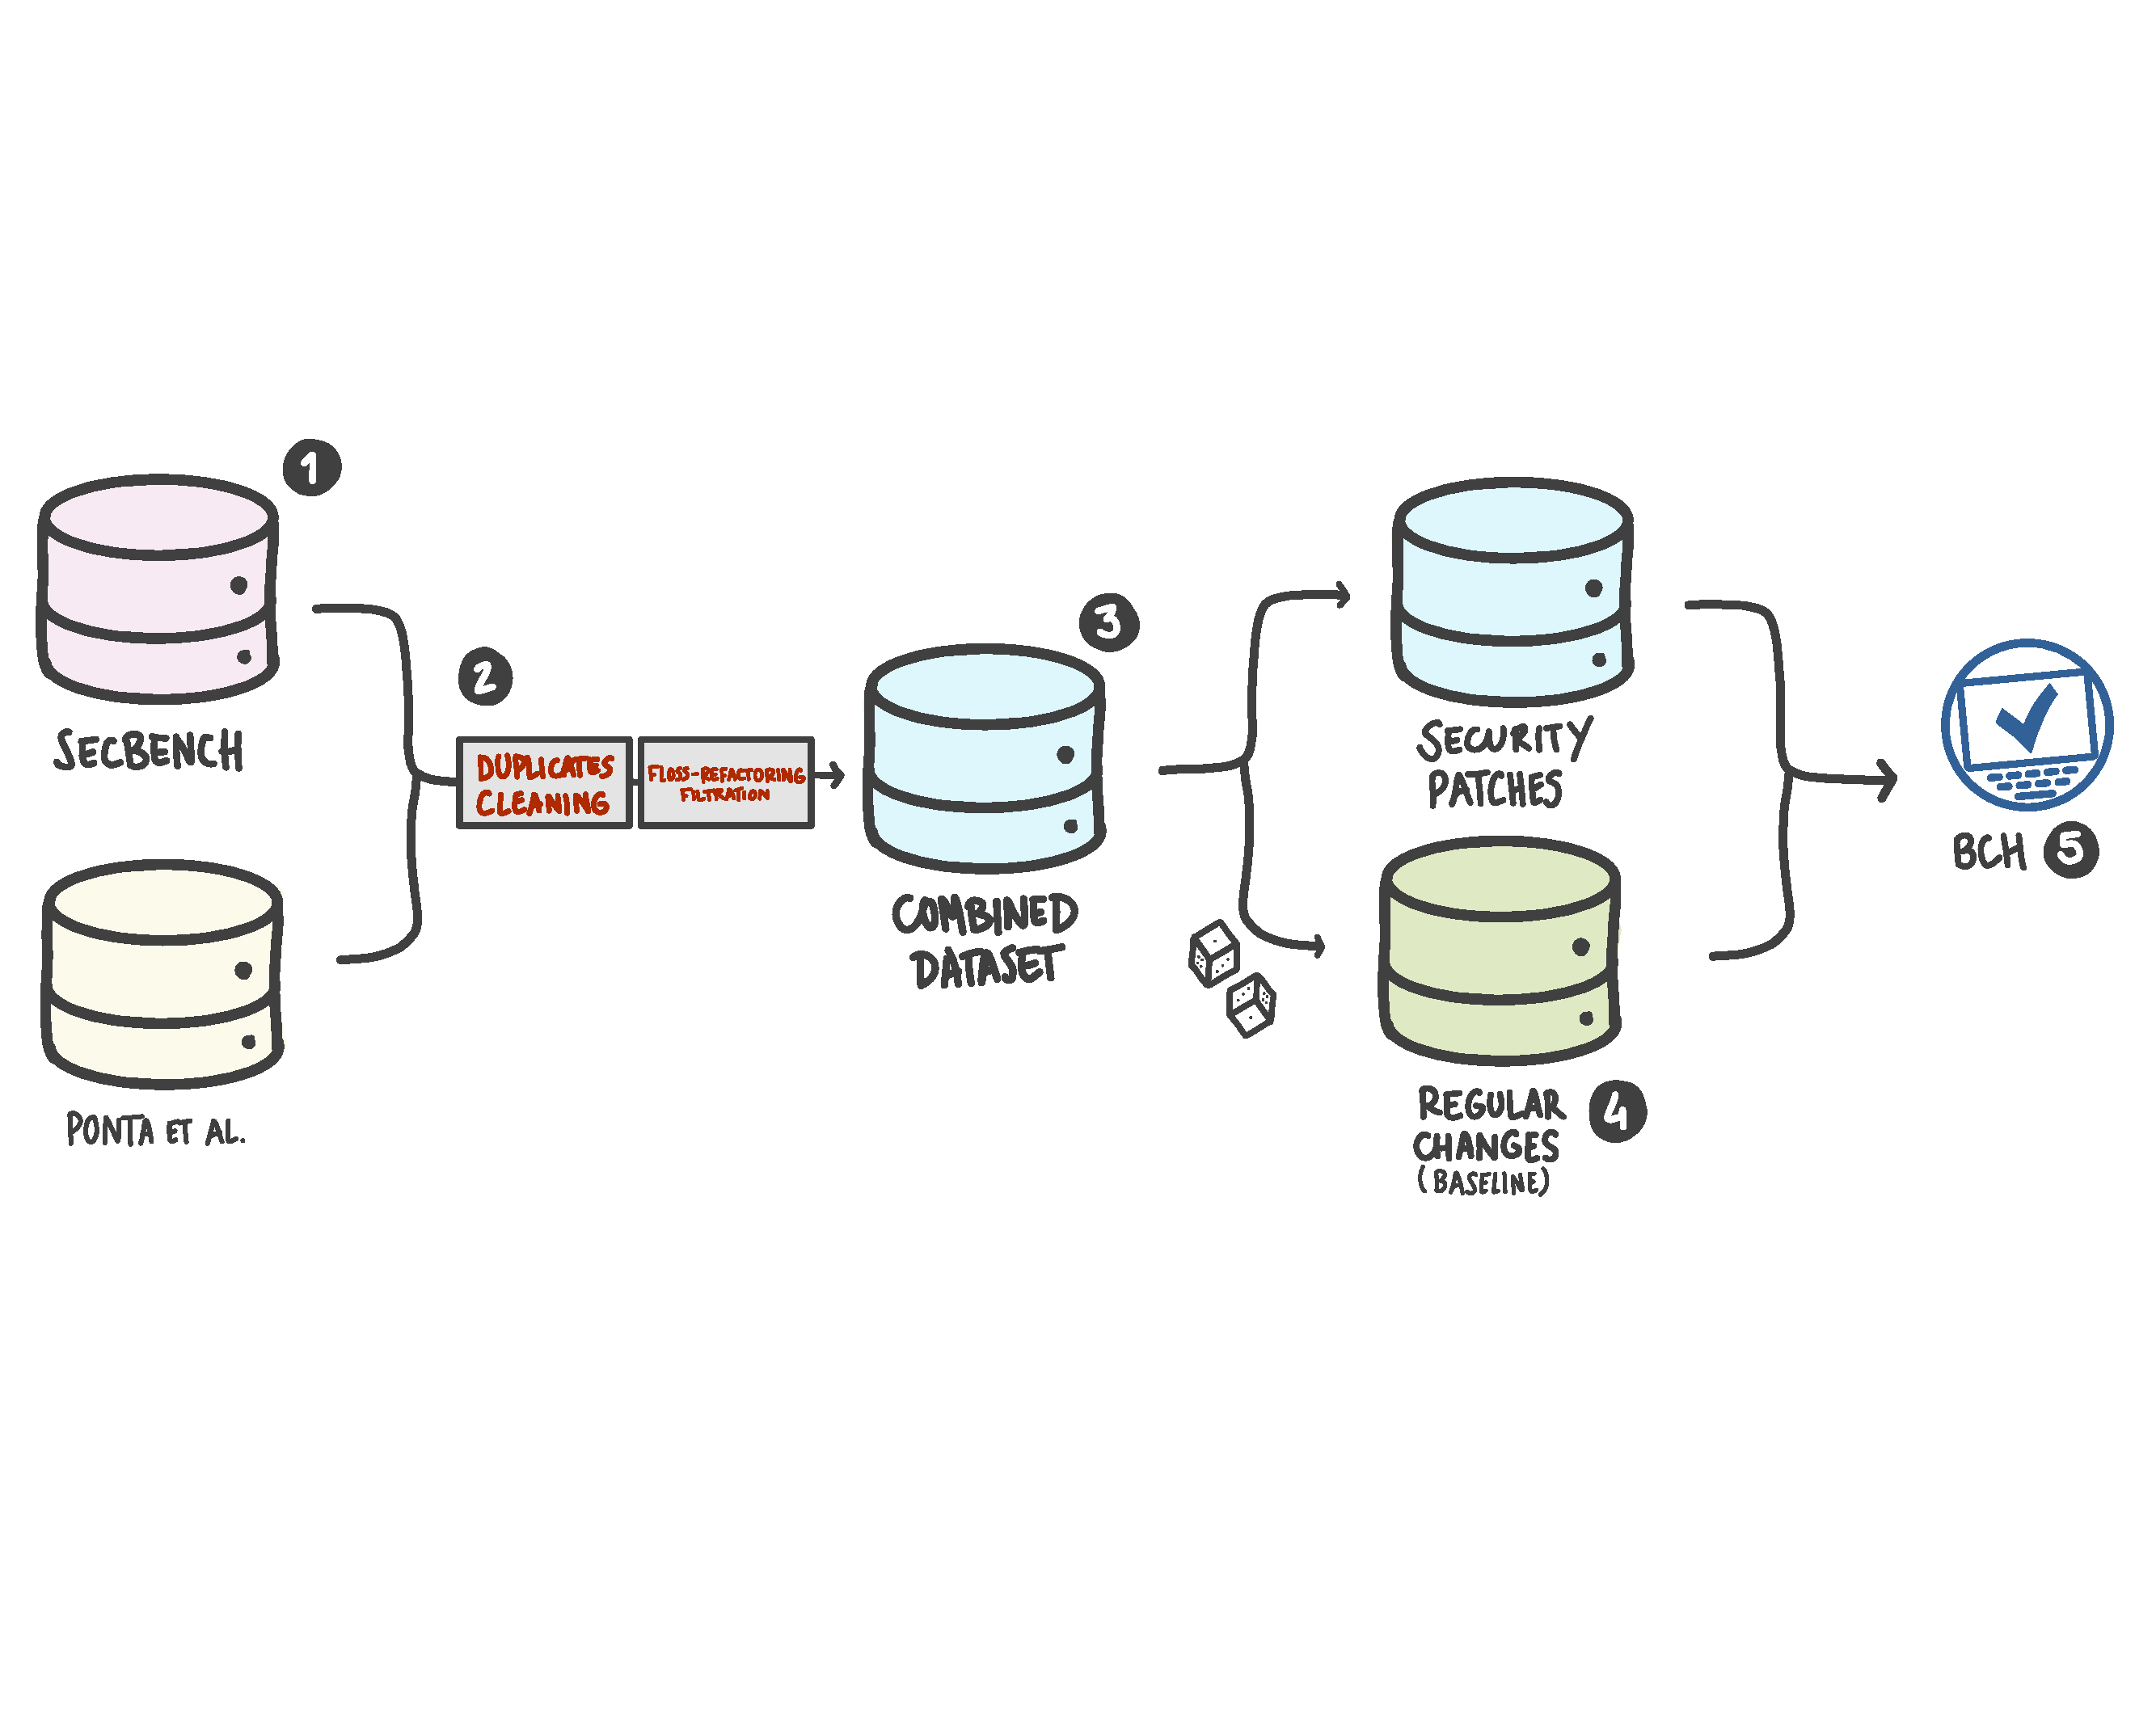
\includegraphics[width=0.45\textwidth]{figures/methodology.pdf}
 	\caption{Study Methodology}
	\label{fig:met}
\end{figure}
%
\subsection{Datasets}
%
To evaluate the impact of security refactorings on the maintainability of
open-source software, we use a combined dataset of security vulnerabilities which is 
the outcome of mining/manually inspect $265$ GitHub projects. Reis and Abreu 
($2017$) mined open-source
software aiming at the extraction of real examples --- created by real
developers --- to test and assess the performance of static analysis tools~\cite{Reis:2017:IJSSE} since
using hand-seeded test cases or mutations could lead to misleading assessments
of the capabilities of the tools~\cite{just2014mutants}. The study yielded a
dataset of $711$ test cases for $16$ different security vulnerability types. Some of the vulnerability types
are based on the OWASP Top $10$ of $2013$~\cite{oswap:2013} and OWASP Top $10$ of
$2017$~\cite{oswap:2017}. Each test case of the
dataset is a triplet: the commit before the patching, the commit responsible
for the patching, and the snippets of code that differ from one version to
another (typically, called \textit{diffs}) --- where one can easily review the
code used to fix the security flaw. 
%
Ponta et al. ($2019$) tracked the \url{pivotal.io} website for vulnerabilities 
from $2014$ to $2019$. For each new vulnerability, the authors manually searched 
for references to commits involved in the patch on the National Vulnerability Database (NVD) website. However, $70\%$
of the vulnerabilities did not have any references to commits. Thus, the authors
used their expertise to locate the commits in the repositories. This technique 
yielded a database of $624$ patches~\cite{10.1109/MSR.2019.00064}. The original 
dataset contains $1282$ commits. One patch can have multiple commits assigned.
To fit the dataset in our methodology, we search for the first and last commits
used to patch the vulnerability. We assumed the last commit of the patch as 
the fix (\emph{sha}) and the parent of the first commit as the vulnerable version 
(\emph{sha-p}).
%
In this study, we focus on computing the
maintainability of the commits before and after the security patching to
evaluate if its impact was positive, negative or none.
The $1335$ patches in the dataset were run against the BCH toolset to
calculate their maintainability reports. However, there are refactorings
discarded from our study due to limitations of BCH: in particular, lack of
language support and project size. The final dataset used in this paper comprises
$998$ security patches. $912$ of these patches are identified with Common Weakness
Enumeration IDs (CWE) where $59.1\%$ were scraped from the National Vulnerability Dataset (NVD) and the remaining $40.9\%$ were manually classified following the \texttt{Research Concepts} view map from the CWE's list.

% In Table~\ref{tab:patterns}, the most prevailing categories are presented. To satisfy the Wilcoxon test size requirement, types of vulnerabilities
% with less than $20$ instances were merged in a bigger group named \textit{Miscellaneous}.

% \begin{table}[h]
% \scriptsize
% 	\caption{Guidelines to produce maintainable code}
% \begin{tabular}{L{1.1cm}L{2.1cm}L{4.3cm}}
%
% \toprule
% \textbf{Pattern} & \textbf{Name} & \textbf{Description}\\
% \midrule
%
% \textbf{CWE-89} &
%  Improper Neutralization of Special Elements used in an SQL Command/SQL Injection (23 cases) &
%  When developers do not keep untrusted data
%      separate from SQL queries. If an attacker sends a command that
%      exploits the syntax of the SQL interpreter, then SQL injection attack is possible.\\\midrule
%
% \textbf{CWE-611} &
%  Improper Restriction of XML External Entity Reference (24 cases) &
% 	XML documents are exchanged through the web containing entities with URIs
%  	that resolve to local/external files. Thus, when XML parsers are not well configured,
%  	attackers have allowed to directly those files.\\\midrule
%
%  \textbf{CWE-20} &
%  Improper Input Validation (76 cases) &
% 	When developers
%  	forget to validate the inputs of an application, attackers may have control
%  	of the control/data flow of the program.\\\midrule
%
%   \textbf{CWE-200} &
% Information Exposure (39 cases)&
% Application's logs are one way of intentional/unintentional disclosure information
%  	to attackers. Many times attackers get access to logs when sould not be authorized to.\\\midrule
%
%    \textbf{CWE-352} &
% Cross-Site Request Forgery/CSRF (22 cases)&
% Poor session tokens generation
%      and management usually allow attackers to send forged HTTP requests
%      including authentication information from the victim to the vulnerable web
%      application.\\\midrule
%
%        \textbf{CWE-264} &
% Permissions, Privileges, and Access Controls (59 cases)&
% Incorrectly
%  	    implemented functionalities related to authentication and session
%  	    management, allowing an attacker to gain access to session tokens,
%  	    passwords, keys, and other sensitive data.\\\midrule
%
%  	           \textbf{CWE-399} &
% Resource Management Errors (22 cases)&
% Resource management issues are found more frequently
%  		in programming languages that do not manage memory automatically (e.g., C/C++
%  	    and Objective-C), i.e., where developers are responsible for
%  	    handling it instead. It is one of the main causes of Denial-of-Service attacks.\\\midrule
%
%  	     	           \textbf{CWE-79} &
% Improper Neutralization of Input During Web Page Generation/Cross-site Scripting (63 cases)&
% Lack of proper validation or escaping
%  	    allows attackers to submit untrusted data to web browsers through malicious
%  	    scripts that can hijack the user sessions or redirect the user to malicious
%  	    sites.\\\midrule
%
%  	     	           \textbf{CWE-22} &
% Improper Limitation of a Pathname to a Restricted Directory/Path Traversal (37 cases) &
% When developers forget to neutralize special elements within the path names to files/directories, attackers
%  	may leverage this flaw to resolve to a location outside of the restricted directory and gain access to documents
%  	or entire repositories.\\\midrule
%
%  	 	     	           \textbf{MISC} &
% Miscellaneous (666 cases) &
% This pattern comprises
%  		several other security refactorings that do not have a CWE assigned and patterns that
%  		do not satisfy the Wilcoxon test size requirement of more than $20$ refactorings.\\
% \bottomrule
% \end{tabular}
% \label{tab:patterns}
% \end{table}

%
% \begin{itemize}
%     \item \textbf{CWE-89: Improper Neutralization of Special Elements used in an SQL Command/SQL Injection (23 cases).} When developers do not keep untrusted data
%     separate from SQL queries. If an attacker sends a command that
%     exploits the syntax of the SQL interpreter, then SQL injection attack is possible.
% %
%     \item \textbf{CWE-611: Improper Restriction of XML External Entity Reference (24 cases).}
% 	XML documents are exchanged through the web containing entities with URIs
% 	that resolve to local/external files. Thus, when XML parsers are not well configured,
% 	attackers have allowed to directly those files.
% %
%     \item \textbf{CWE-20: Improper Input Validation (76 cases).} When developers
% 	forget to validate the inputs of an application, attackers may have control
% 	of the control/data flow of the program.
% %
%     \item \textbf{CWE-200: Information Exposure (39 cases).} Application's logs are one way of intentional/unintentional disclosure information
% 	to attackers. Many times attackers get access to logs when sould not be authorized to.
% %
% 	\item \textbf{CWE-352: Cross-Site Request Forgery/CSRF (22 cases).} Poor session tokens generation
%     and management usually allow attackers to send forged HTTP requests
%     including authentication information from the victim to the vulnerable web
%     application.
% %
% 	\item \textbf{CWE-264: Permissions, Privileges, and Access Controls (59 cases).} Incorrectly
% 	    implemented functionalities related to authentication and session
% 	    management, allowing an attacker to gain access to session tokens,
% 	    passwords, keys, and other sensitive data.
% %
% 	\item \textbf{CWE-399: Resource Management Errors (22 cases).} Resource management issues are found more frequently
% 		in programming languages that do not manage memory automatically (e.g., C/C++
% 	    and Objective-C), i.e., where developers are responsible for
% 	    handling it instead. It is one of the main causes of DoS attacks.
% %
% 	\item \textbf{CWE-79: Improper Neutralization of Input During Web Page Generation/Cross-site Scripting (62 cases)} Lack of proper validation or escaping
% 	    allows attackers to submit untrusted data to web browsers through malicious
% 	    scripts that can hijack the user sessions or redirect the user to malicious
% 	    sites.
% %
% 	\item \textbf{CWE-22: Improper Limitation of a Pathname to a Restricted Directory/Path Traversal (37 cases).}  When developers forget to neutralize special elements within the pathnames to files/directories, attackers
% 	may leverage this flaw to resolve to a location outside of the restricted directory and gain access to documents
% 	or entire repositories.
% %
% 	\item \textbf{Miscellaneous (673 cases)} This pattern comprises
% 		several other security refactorings that do not have a CWE assigned and patterns that
% 		do not satisfy the Wilcoxon test size requirement of more than $20$ refactorings.
% \end{itemize}
%
\subsection{Security vs. Baseline Commits}
%
Previous studies attempted to measure the impact of regular refactorings on
open-source software maintainability~\cite{HEGEDUS2018313}. However, there is no
previous work focused on comparing the impact of security refactorings with
regular refactorings on maintainability.
We analyze the maintainability of regular commits (i.e., commits not related
to security fixes) and use them as a baseline.

The baseline dataset uses the security commits dataset as input.
Both datasets have the same size. For each
security commit, a commit with an approximate size is searched. Due to the complexity 
of some patches, it was not possible to find patches with the exact number of added and 
deleted lines. Our search uses the patch \emph{diff} to look for a new similar \emph{diff}. The algorithm integrates the following steps:

\begin{enumerate}
\item Calculates the \emph{diff} between the security patch commit (\emph{sha}) and its parent (\emph{sha-p}).
\item Selects a random commit from the project (\emph{sha-reg}).
\item Calculates the \emph{diff} between the random commit (\emph{sha-reg}) and its parent (\emph{sha-reg-p}).
\item Checks if the size from the regular change has the same/approximated size to 
the security patch.
\end{enumerate}

\Sof{The pair of the random commit and its parent is accepted if the \emph{diff} 
size fits in the range size considered acceptable at the moment. The algorithm 
starts with a step of $1$. Every $10$ attempts to search for a change with the 
same \emph{diff} the step increases. Thus, if a change suffered $20$ deletions 
and $10$ additions, then, in the first $10$ attempts, the algorithm searches 
for a \emph{diff} with deletions between $19$ and $21$ and additions between 
$9$ and $11$. After the $10$ first attempts, the algorithm increase the step 
for $2$ and searches for a \emph{diff} with deletions between $18$ and $22$ 
and additions between $8$ and $10$. We originate the regular commits from the 
security commits to ensure that differences in maintainability are not a 
consequence of characteristics of different projects.}

\subsection{Maintainability Analysis}

In this research, we follow a very similar methodology to the one presented 
in previous work on the maintainability of energy-oriented fixes~\cite{cruz2019energyoriented}. 
As said before, the web-based source code analysis service \emph{Better Code
Hub} (BCH) is used to collect the maintainability reports of the refactorings of
each project. Table~\ref{tab:guidelines} presents the $10$ guidelines $-$ proposed
by BCH's authors for delivering software that is not difficult to
maintain~\cite{Visser:2016:OREILLY} $-$ and maps each guideline to the metric 
calculated by BCH. Theses guidelines are calculated using the metrics 
presented in~\cite{criteria:2017} and also briefly explained on Table~\ref{tab:guidelines}. 
During each guideline evaluation, the tool determines the compliance towards 
one guideline by establishing limits for the percentage of code allowed to be 
in each of the $4$ risk severity levels
(\emph{low risk}, \emph{medium risk}, \emph{high risk}, and \emph{very high
risk}). If the project does not violate the thresholds, then it is compliant
with the guideline. These thresholds are calibrated by BCH using their own
data/experience --- using open-source and closed software systems. If a project is
compliant with a guideline, it means that it is at least $65\%$ better than the
software used by BCH to calculate the thresholds\footnote{Check the answer to
\emph{How can I adjust the threshold for passing/not passing a guideline?} at
\url{https://bettercodehub.com/docs/faq} (Accessed on \today{})}.

\begin{figure}[h]
 	\centering 	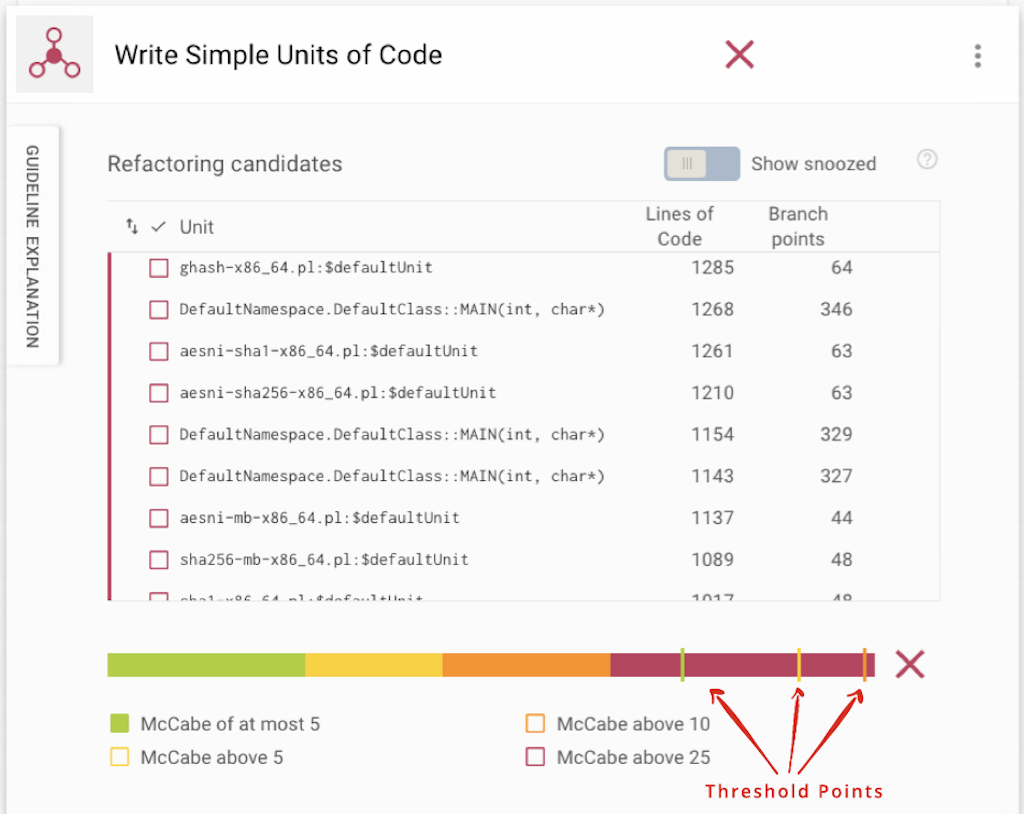
\includegraphics[width=0.44\textwidth]{figures/bch_report.png}
 	\caption{Maintainability report of OpenSSL's CVE-$2014$-$3506$ vulnerability
refactoring for the guideline \emph{Write Simple Units of Code} provided by
\emph{Better Code Hub}. This version of OpenSSL does not comply with the
guideline in the example since the bars do not reach the threshold points. This
example only complies with $\sfrac{1}{10}$ guidelines (\emph{Write Clean Code}).}
	\label{fig:bchrep}
\end{figure}

\begin{table}[h]
\scriptsize
	\caption{Guidelines to produce maintainable code}
\begin{tabular}{L{1.66cm}L{3.3cm}L{2.7cm}}

\toprule
\textbf{10 Guidelines} & \textbf{Description} & \textbf{Metric}\\
\midrule

\textbf{Write Short Units of Code} & Limit code units to $15$ LOCs because smaller
 units are easier to understand, reuse and test them & \textbf{Unit Size:} \% of 
 LOCs within each unit~\cite{criteria:2017} \\\midrule

\textbf{Write Simple Units of Code} & Limit branch points to $4$ per unit because
it makes units easier to test and modify & \textbf{McCabe Complexity:} \# of decision 
points~\cite{1702388,criteria:2017}\\\midrule

\textbf{Write Code Once} & Do not copy code because bugs tend to replicate at
multiple places (inefficient and error-prone) & \textbf{Duplication:} \% of redundant 
LOCs~\cite{criteria:2017}\\\midrule

\textbf{Keep Unit Interfaces Small} & Limit the number of parameters to at most
$4$ because it makes units easier to understand and reuse & \textbf{Unit Interfacing:} 
\# of parameters defined in a signature of a unit~\cite{criteria:2017} \\\midrule

\textbf{Separate Concerns in Modules} & Avoid large modules because changes in
loosely coupled databases are easier to oversee and execute & \textbf{Module Coupling:} \# of
incoming dependencies~\cite{criteria:2017} \\\midrule

\textbf{Couple Architecture Components Loosely} & Minimize the amount of code
within modules that are exposed to modules in other components & \textbf{Component Independence:} 
\% of code in modules classified as hidden~\cite{criteria:2017}\\\midrule

\textbf{Keep Architecture Components Balanced} & Balancing the number of
components ease locating code and allow for isolated maintenance & \textbf{Component Balance:} 
Gini coefficient to measure the inequality of distribution between components~\cite{criteria:2017} \\\midrule

\textbf{Keep your code base Small} & Reduce and avoid the system size because
small products are easier to manage and maintain & \textbf{Volume:} \# of LOCs converted 
to man-month/man-year~\cite{criteria:2017} \\\midrule

\textbf{Automate Tests} & Test your code base because it makes development
predictable and less risky & \textbf{Testability:} Ratings aggregation $-$ unit 
complexity, component independence and volume~\cite{Visser:2016:OREILLY}
 \\\midrule

\textbf{Write Clean Code} & Avoid producing software with code smells because
it is more likely to be maintainable in the future & \textbf{Code Smells:} 
\# of Occurrences~\cite{Visser:2016:OREILLY} (e.g., magic constants and long 
identifier names) \\
\bottomrule
\end{tabular}
\label{tab:guidelines}
\end{table}


Figure~\ref{fig:bchrep} shows an example of the report
provided by BCH for a project after finishing its evaluation. The example
refers to the OpenSSL CVE-$2014$-$3506$ vulnerability refactoring ---
as described by Section~\ref{sec:motivation}. This
version of OpenSSL only complies with $1$ out of $10$ guidelines: \emph{Write
Clean Code}.

\Sof{SIG defines \emph{Units} as the smallest groups of code that can be maintained
and executed independently~\cite{Visser:2016:OREILLY} (e.g., methods and
constructors in Java). One of the guidelines with which the project does not
comply is the one presented in the report (cf. Figure~\ref{fig:bchrep}):
\emph{Write Simple Units of Code}. BCH analyzes this guideline based on the
McCabe Complexity~\cite{1702388} to calculate the number of branch points of a
method. The bar at the bottom of the figure represents the top $30$ units that
violate the guideline, sorted by severity. The violation severities are
indicated using colors, and there is a legend to help to interpret them. The
green bar represents the number of compliant branch points per unit (\emph{at
most $5$}), i.e., the number of units are compliant with ISO
$25010$~\cite{iso:2011}. Yellow, orange and red bars represent units that do not
comply with medium (\emph{above $5$}), high (\emph{above $10$}) and very high
(\emph{above $25$}) severity levels. In the bar, there are marks that pinpoint
the compliance thresholds for each severity level. If the green mark is
somewhere in the green bar it means it is compliant with a low level of
severity.}

\begin{figure}[h]
 	\centering 	
	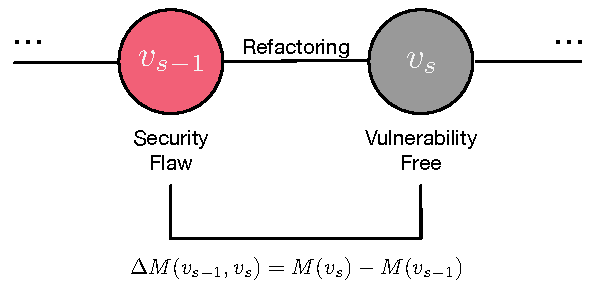
\includegraphics[width=0.6\linewidth]{figures/commit.pdf}
 	\caption{Maintainability difference for security commits}
	\label{fig:commit}
\end{figure}

Aiming to analyze the impact of security patches, we use BCH to compute the
maintainability of two different versions of the project (cf. Figure~\ref{fig:commit}):

\begin{itemize}
	\item $v_{s-1}$, the version containing the security flaw, i.e., before the
	patch (\emph{sha-p});
	\item $v_{s}$, the version free of the security flaw, i.e., after the
	patch (\emph{sha});
\end{itemize}

Patches can be performed through one commit, several consecutive commits, or 
commit(s) interleaved with more programming activities, being the later
commonly called a floss-refactoring. This study considers mainly 1-commit 
patches. Yet, a small percentage of data points had more than one commit 
involved in the patch. We manually inspected these cases and $23$ 
floss-refactorings were identified and disregarded since it would not
be fair to measure the maintainability of these cases where other
programming activities are involved.

The BCH tool does not compute the final score that our study needs to compare
maintainability amongst different project versions. For this, we follow previous 
work on measuring the impact of energy-oriented 
refactorings~\cite{cruz2019energyoriented}. Luis et al. ($2019$) proposed an 
equation to capture the distance between the current state of the project and
the standard thresholds calculated by the BCH based on the insights provided 
in~\cite{Olivari:2018}. The equation provided in~\cite{cruz2019energyoriented} 
considers that the size of project changes does not affect the maintainability 
and that the distance to lower severity levels is less penalized than to the
thresholds in high severity levels.

% 	thresholds in high severity levels
% 	difference between two versions
% The equation considers the following:
% \begin{itemize}
% 	\item \textbf{Size of project changes does not affect the maintainability
% 	difference between two versions, $\Delta M (v_{s-1},v_{s}) = M(v_{s}) - M(v_{s-1})$.} We
% 	aim at evaluating security patterns occurring in different projects similarly.
% 	Thus, the derived metric uses the \textit{raw} number of lines of code rather
%   percentages for normalization purposes.
% 	\item \textbf{Distance to lower severity levels is less penalized than to the
% 	thresholds in high severity levels.} Severity level weights based on the
% 	severity level to count lines of code that violate maintainability guidelines.
% \end{itemize}


Given the violations for the BCH guidelines, the maintainability score is computed
$M(v)$ as follows:

\begin{equation}
    M(v) = \sum_{g \in G}^{} M_{g}(v)
\end{equation}

\noindent
where $G$ is the group of maintainability guidelines from BCH
(Table~\ref{tab:guidelines}) and $v$ is the version of the software under
evaluation. $M(v) < 0$ indicates that version $v$ is violating (some of) the
guidelines, while $M(v) > 0$ indicates that version $v$ is following
the BCH guidelines. The maintenance for the guideline $g$, $M_g$ for a given version
of a project is computed as the summation of the compliance with the 
maintainability guideline for the given severity level (medium, high, and very high).
\Sof{The compliance for a severity level
is calculated based on the number of lines of code that comply and not comply
with the guideline at a given severity level as explained in more
detail in previous work~\cite{cruz2019energyoriented}.} In our analysis, we compute 
the difference of maintainability between the security commit ($v_{s}$) and its parent 
commit ($v_{s-1}$), as illustrated in Figure~\ref{fig:commit}. Thus, we can determine 
which patches had a positive, negative or null impact on the project maintainability. 


\Sof{@todo: Don't forget to mention the limitations of BCH and the outliers.}

% The compliance $C$ for a given severity
% level $l$ is derived by:
%
% \begin{equation}\label{eq:3}
%     C(l) = LOC_{compliant}(l) - w(l) * LOC_{\neg compliant}(l)
% \end{equation}
%
% \noindent
% where $LOC_{compliant}(l)$ are the lines of code that comply with the guideline
% at the given severity level $l$, $LOC_{\neg compliant}(l)$ are the lines of code
% that do not comply with the guideline at the given severity level $l$ and $w(l)$
% is the weight factor to heighten the impact of non-compliant lines in comparison to
% compliant lines. Finally, the term $w(l)$ is calculated as follows:
%
% \begin{equation}
%     w(l) = \frac{1 - \theta(l)}{\theta(l)}
% \end{equation}
%
% \noindent
% where $\theta(l)$ is the threshold in percentage of the lines of code that are
% accepted to be non-compliant with the guideline for the severity level $l$. This
% is a standard value defined by BCH. In other words, the factor $w$ is used in
% Equation~\ref{eq:3} to highlight the lines of code that are not complying with
% the guideline. Then, we compute the difference of maintainability between the
% security commit ($v_{s}$) and its parent commit ($v_{s-1}$), as illustrated in
% Figure~\ref{fig:commit}.

\subsection{Statistical Validation}\label{sec:statsval}
%
To validate the maintainability differences in different groups of commits
(e.g., baseline and security commits), we use the Paired Wilcoxon signed-rank
test with the significance level $\alpha = 0.05$~\cite{10.2307/3001968}. In
other words, we test the null hypothesis that the maintainability difference
between pairs of versions $v_{s-1}$, $v_s$ (i.e., before and after a
security-commit) come from the same distribution. Nevertheless, this test 
has a limitation: it does not consider the groups of commits with a 
zero-difference maintainability. In $1959$, Pratt provided an improvement to 
the test to solve this issue making the test more robust. Thus, we use a 
version of the Wilcoxon test that incorporates the cases where 
maintainability is different from zero~\cite{10.2307/2282543}.
The Wilcoxon test requires a distribution size of at leat $20$ instances.
To understand the effect-size, as advocated by the Common-language effect 
sizes\cite{graw:1992}, we compute the mean difference, the median of the 
difference, and the percentage of cases that reduce maintainability.
%
\section{Results \& Discussion}\label{sec:results}

This study evaluates a final total of $998$ security and baseline commits 
from $262$ distinct open-source projects. The following section presents and 
discusses the results for each question. Research questions are also answered.

\textit{\textbf{RQ1: What is the impact of security patches on the
maintainability of open-source software?}}
\textit{Patching vulnerabilities may harm the maintainability of open-source
software.}

In this section, we report and discuss the impact of patches on open-source
software maintainability under four different views: guidelines/metrics, 
severity, programming language and formula proposed - the mean of all 
guidelines/metrics.

% As expected, vulnerabilities with higher severity are more likely to impact negatively
% the maintainability of software. This suggests that high/medium severity vulnerabilities may
% need more attention than low severity when patching vulnerabilities.
% %
% We would expect that the negative impact of programming languages on
% maintainability to be more severe, as arguably poor design of programming
% languages and lack of using the best practices lead to more buggy and vulnerable
% code~\cite{Ray:2017:LSP:3144574.3126905, 2019arXiv190110220B}. However,
% Figure~\ref{fig:lang_main} shows that only \emph{C/C++} and \emph{Python} have a negative impact approximate to $50\%$ on software maintainability. We suspect that these values are
% the result of projects contributions policies. Nine of the top-10 of dataset projects
% with more contributors have restrict contribution policies regarding code
% standards. Some examples are the \texttt{laravel/framework},
% \texttt{php/php-src}, \texttt{openssl/openssl} and \texttt{cakephp/cakephp}. For
% instance, \texttt{laravel/framework} requires the \texttt{PSR-2
% Standard}\footnote{PSR-2 Standard available at
% \url{https://www.php-fig.org/psr/psr-2/} (Accessed on \today{})} that is a coding style guide for \texttt{PHP}.

\textbf{Guidelines/Metrics:} Each patch performs a set of changes
on the source code of the software. These changes may have a different
impact on the guidelines/metrics used to measure software maintainability. 
Figure~\ref{fig:guidelines} shows the impact of security patches 
on each guideline individually. Under each guideline is stated the 
metric used to the calculations. Table~\ref{tab:guidelines} describes 
in more detail the metrics behind the guidelines presented. 
For each type of guideline, three types of impact of patches in 
the software maintainability are presented: 
\emph{negative}, maintainability decreases (\emph{red});
\emph{none}, maintainability remains the same (\emph{yellow}); and,
\emph{positive}, maintainability increases (\emph{green}). Next to each
type of guideline, it is presented the mean ($\overline{x}$) and median (M)
of the maintainability difference and the p-value resulting from the
Paired Wilcoxon signed-rank test.

Regarding the impact of security patches for each guideline, we observe
that overall patches have a more positive impact than negative in
all guidelines/metrics. However, patching vulnerabilities also has a very
significant negative impact on all guidelines - between $10\%$ and $40\%$. 
\emph{Write Simple Units of Code} ($37.3\%$), \emph{Write Short Units of 
Code} ($37.6\%$) and \emph{Separate Concerns in Modules} ($33.2\%$) are the 
most affected guidelines. This may imply that developers when patching 
vulnerabilities fail to design/implement solutions that continue to respect 
the limit bounds of branch points (/programming conditions) and function/module 
sizes (e.g., functions should not have more than $15$ LOCs). Still, on 
respecting bound limits, developers also seem to not consider the limit 
of $4$ parameters per function for the \emph{Keep Unit Interfaces Small} 
guideline required by BCH, in $24.5\%$ of the cases. This guideline is usually
violated when the patch requires to input new information to a function/class 
and developers fail to use the \emph{Introduce Parameter Object} refactoring 
pattern. Results do not provide statistical significance to the \emph{Separate 
Concerns in Modules} guideline, i.e., results should be read carefully. 

Software architecture is also affected while patching vulnerabilities.
Both \emph{Couple Architecture Component Loosely} and \emph{Keep
Architecture Components Balanced} guidelines suffer a negative impact of 
$26.7\%$ and $11.1\%$, respectively. Component independence and balance
are important to make easier to find the source code developers
want to patch/improve and to understand how the high-level components
interact with others. However, results may imply that developers
fail to use techniques such as encapsulation to hide implementation
details and make the system more modular.

Software systems typically have $9\%$-$17\%$ of cloned code~\cite{5773403}. 
The \emph{Write Code Once} guideline results show that duplicated code 
increased in $174$ ($17.4\%$) of the patches. Previous work showed a 
correlation between code smells and code duplication~\cite{7476787} 
which may also be reflected in the \emph{Write Clean Code} guideline results. 
BCH reported new code smells for $152$ ($15.2\%$) patches which according 
to previous work may harm software security since some of these new code
smells may be new vulnerabilities~\cite{8819456}. Thus, while developers 
tend to ignore refactoring techinques such as the \emph{Replace Method 
with Method Object} technique, they may also be introducing new software 
vulnerabilities. 
  
For projects with large codebases, the results retrieved for \emph{Keep Your 
Codebase Small} were not viable because they retrieved values above the limit 
set by BCH ($20$ Person-years). The \emph{Automated Tests} guideline was also 
not considered because the BCH tool does not return the same type of information
as for other guidelines. Due to BCH limitations, we detected a few data points
that retrieved incorrect overall calculations for one version of the software. 
Those data points were disregarded from the study.

Although overall patching vulnerabilities has a less negative impact, it is 
important to note that the design debt of one guideline can lead
to severe impacts on the software quality~\cite{10.1145/1985362.1985366} 
and in the market value of a company~\cite{4267025}. Thus,
tools like Better Code Hub and static analysis should be leveraged to 
assess the risk of patching vulnerabilities - alongside with pull
requests and code reviews. While style-guided static code analysis
may be daunting due to the amount of rules and different effects
on maintainability, BCH ensures that the $10$ chosen guidelines are
the ones with the highest effect on maintainability. 
%
% 
 \begin{figure}[H]
  	\centering
 	\vspace{-0.3 cm}
  	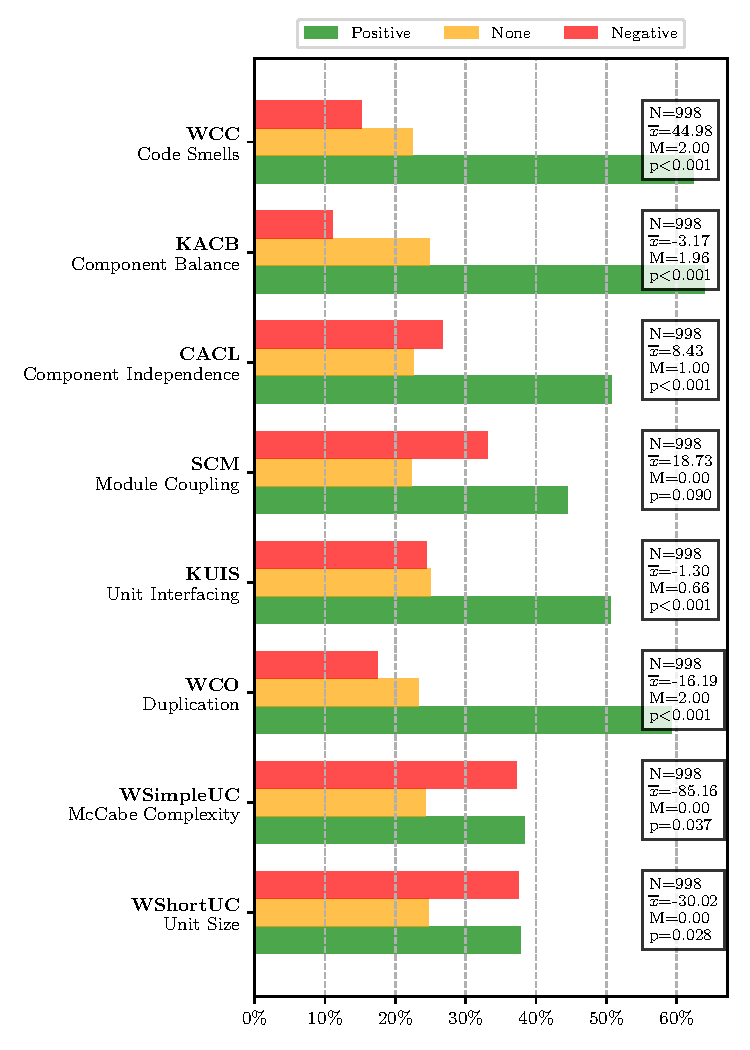
\includegraphics[width=0.45\textwidth]{figures/main_per_guideline.pdf}
 	\vspace{-0.3 cm}
  	\caption{Impact of the security patches per guideline.}
 	\label{fig:guidelines}
 	\vspace{0.2 cm}
 	\scalebox{0.5}{
 	\begin{tabular}{r@{: }l r@{: }l}
 	$WCC$ & Write Clean Code & $KACB$ & Keep Architecture Components Balanced\\
 	$CACL$ & Couple Architecture Components Loosely & $SCM$ & Separate Concerns 
	in Modules \\
 	$KUIS$ & Keep Unit Interfaces Small & $WCO$ & Write Code Once \\
 	$WSimpleUC$ & Write Simple Units of Code & $WShortUC$ & Write Short Units of 
	Code
 	\end{tabular}
 	}	
 \end{figure}
 
\textbf{Severity:} Some of the vulnerabilities are identified with \emph{Common 
Vulnerabilities and Exposure} (CVE) entries. We leveraged the \emph{National Vulnerability 
Database} (NVD) website to obtain their severity levels. In total, we 
retrieved severity scores for $551$ vulnerabilities: $117$ (\emph{HIGH}), 
$404$ (\emph{MEDIUM}) and $30$ (\emph{LOW}). Figure~\ref{fig:severity} 
presents the impact of security patches per severity level on the 
maintainability of open-source software. We observe that patches for 
\emph{HIGH} ($47.9\%$) and \emph{MEDIUM} ($44.1\%$) severity vulnerabilities 
hinder more the maintainability of software than \emph{LOW} ($30.0\%$) 
severity vulnerabilities. Again, patches have a considerable 
negative impact on software maintainability - between $30\%$ 
and $50\%$. None statistical significance was retrieved. However, 
results should not be disregarded because they seem to confirm the 
assumption that higher severity vulnerabilities patches may have a 
more negative impact on maintainability.

\begin{figure}[h]
 	\centering 	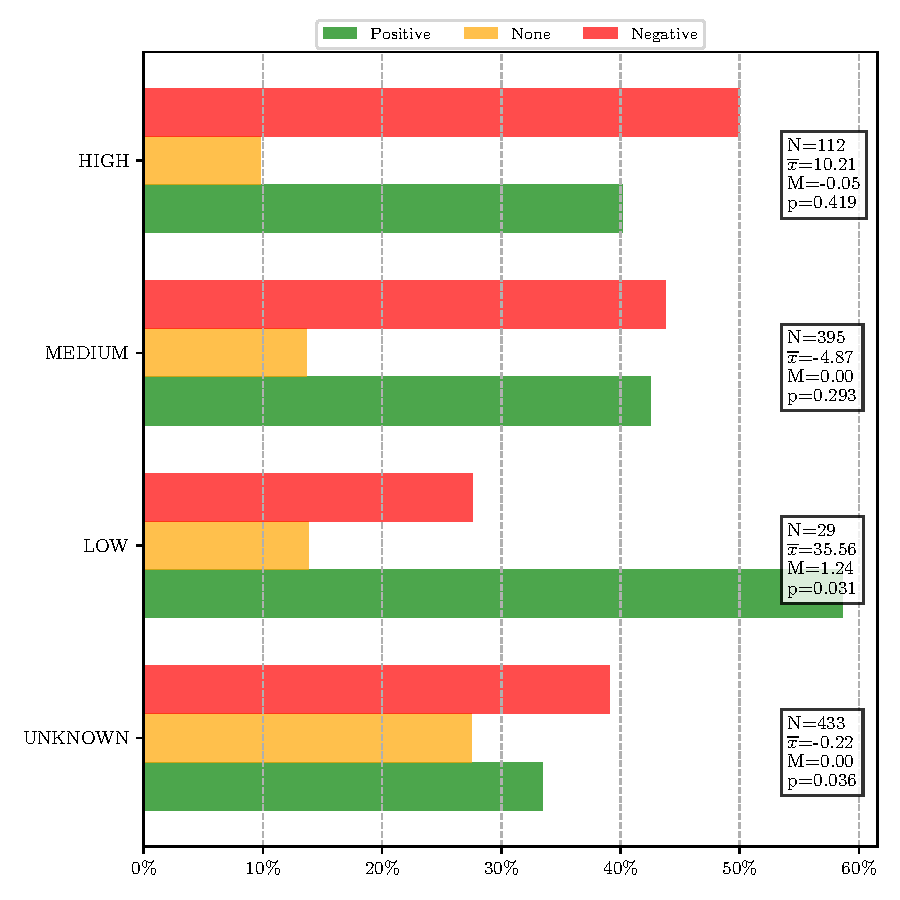
\includegraphics[width=0.4\textwidth]{figures/main_per_severity.pdf}
 	\caption{Maintainability difference by vulnerability severity.}
	\label{fig:severity}
\end{figure}

\textbf{Programming Languages:} We have also evaluated the impact on the maintainability per programming 
language of open-source software (Figure~\ref{fig:lang_main}). We restrict 
this analysis to programming languages with at least $20$ data points, as this 
is a requirement for our hypothesis tests. Thus, we compare the results for 
\texttt{C/C++}, \texttt{Ruby}, \texttt{Java}, \texttt{Objective C/C++}, 
\texttt{Python} and \texttt{PHP}. The remaining languages are included into 
\texttt{Other}. \texttt{C/C++} ($46.54\%$), \texttt{Ruby} ($46.48\%$) and 
\texttt{PHP} ($38.27\%$) are the programming languages with a more negative
impact on the maintainability of software. \texttt{Java} seems to be the 
language less affected by patching, more than $50\%$ of patches had a positive 
impact on maintainbility. But overall patches in all languages have a 
considerable negative impact on maintainability - from $30\%$ to $50\%$ - which 
confirms the need for better and more secure programming languages. 
Statistical significance was only retrieved for the \texttt{C/C++} 
(p-value = $2.24$x$10^{-05}$) and \texttt{Ruby} (p-value = $0.041$) languages.
Results should be read with care where statistical significance was not found.
Yet, data reports very interesting hints on the impact of programming languages 
on security patches.

\begin{figure}[h]
  \centering
  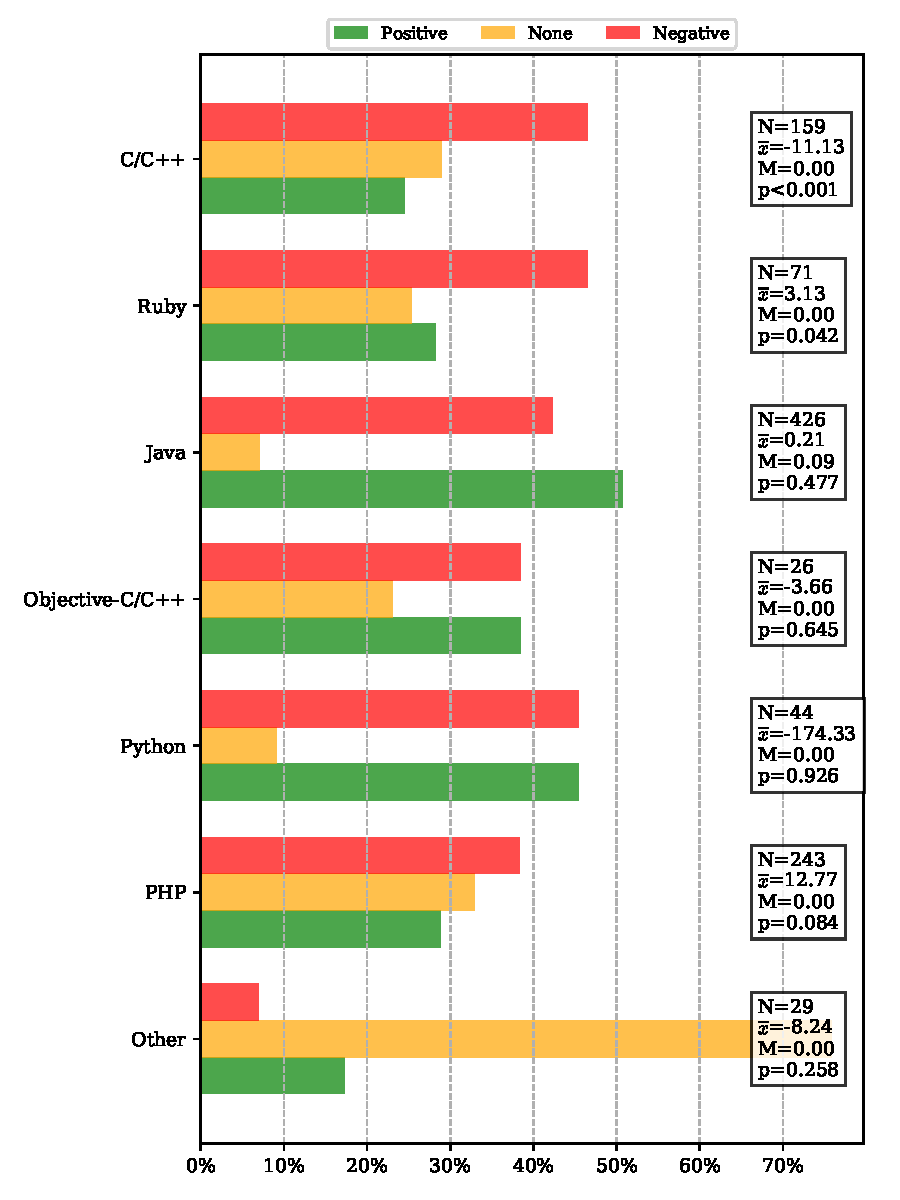
\includegraphics[width=0.4\textwidth]{figures/main_per_language.pdf}
  \caption{Maintainability difference by programming language.}
  \label{fig:lang_main}  
\end{figure}

% Following the \textit{American Statistical Association}
% recommendations~\cite{doi:10.1080/00031305.2016.1154108}, we consider the results for
% Ruby as statistically significant because its p-value is on the borderline.

\textbf{Formula:} Maintainability is being calculated as the mean of 
the guidelines computed by Better Code Hub (BCH). Regarding security 
commits results (Figure~\ref{fig:secvsreg}), we observe that
maintainability decreases in $41.28\%$ ($412$), remains the same in $20.64\%$ 
($206$) and increases in $38.08\%$ ($380$) of the cases. The resulting
p-value of the Paired Wilcoxon signed-rank test is $0.044$. Since the p-value is 
below the significance level of $0.05$, we argue that \emph{security patches 
have a negative impact on the maintainability of open-source software}.
%

\textit{\textbf{RQ2: Which weaknesses are more likely to
affect open-source software maintainability?}}

\begin{figure*}[htp]
  \centering
  \subfigure[Maintainability difference by first-level weaknesses from the 
  \textit{Research Concepts} list on Common Weakness Enumeration (CWE)]{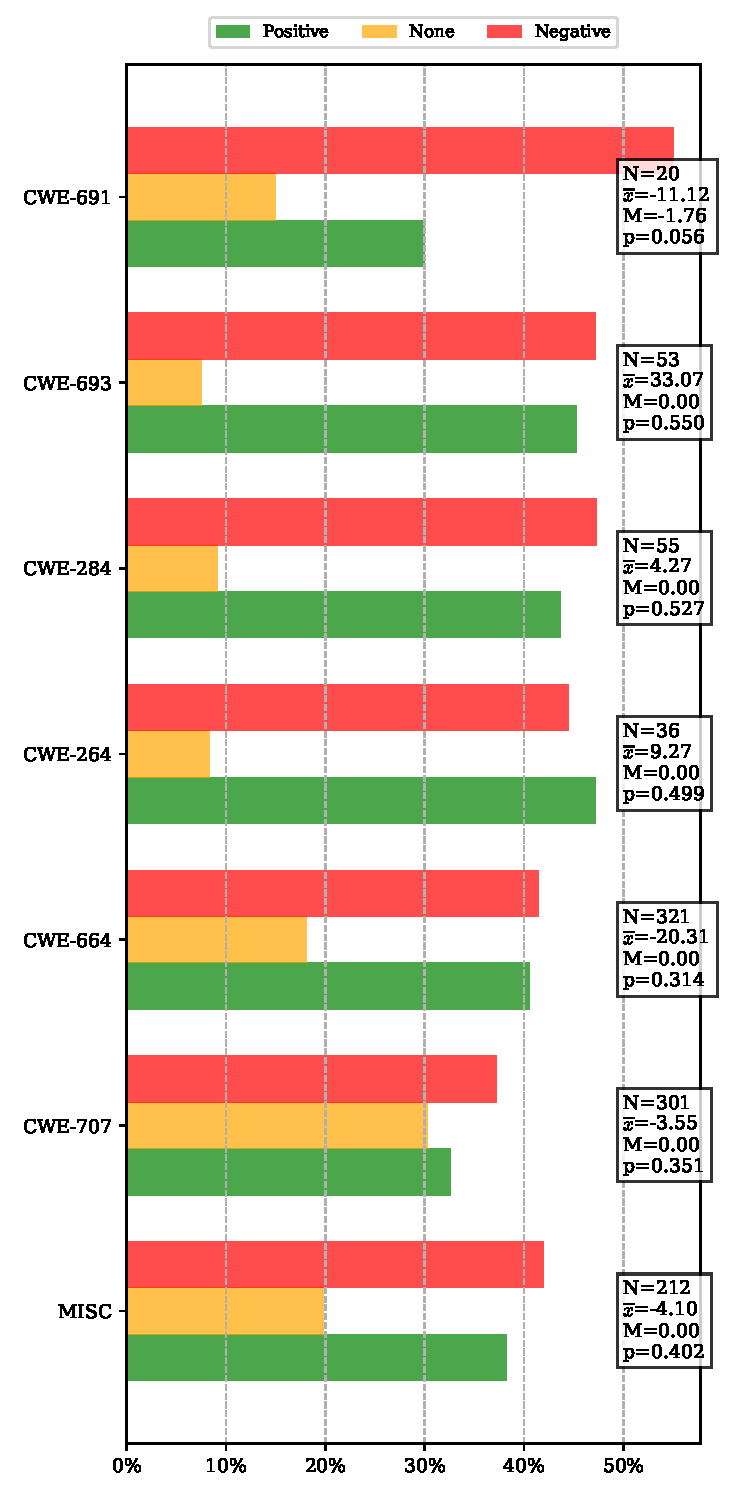
\includegraphics[scale=0.4]{figures/main_per_cwe.pdf}}\quad\quad
  \subfigure[Maintainability difference by sub-weaknesses of the 
  \textit{Improper Neutralization} Weakness (CWE-707)]{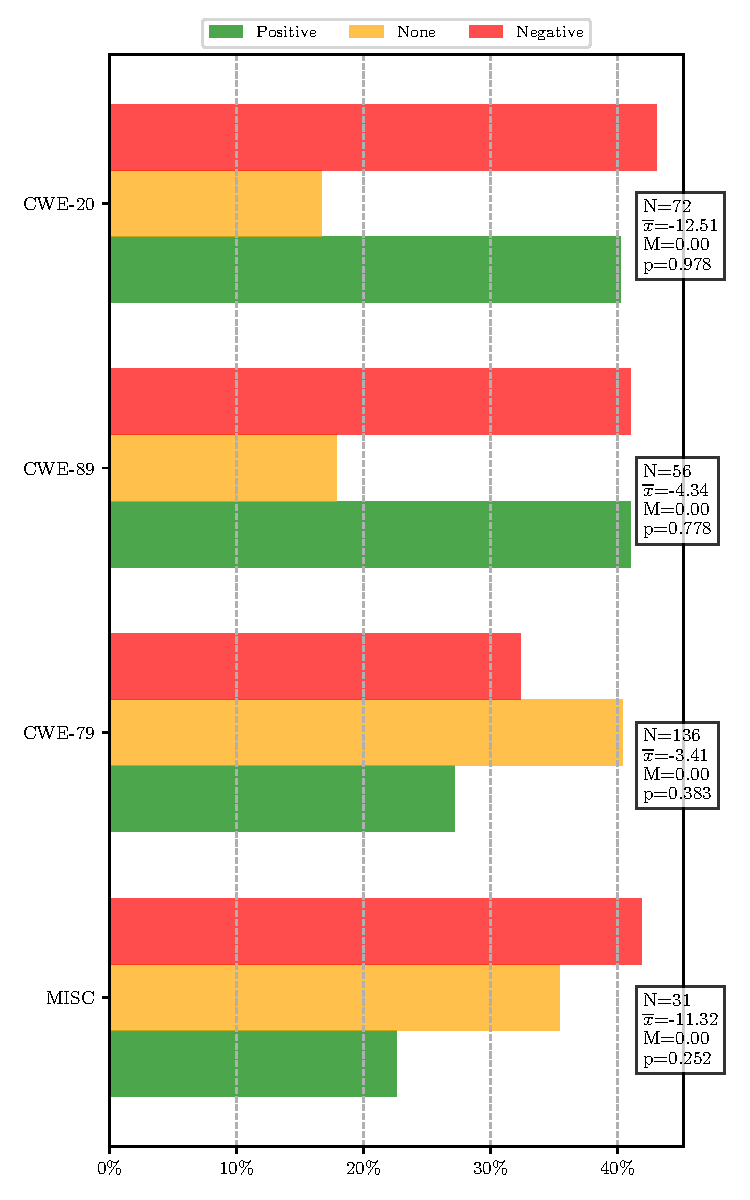
\includegraphics[scale=0.4]{figures/main_per_cwe_spec_707.pdf}}\quad\quad
    \subfigure[Maintainability difference by sub-weaknesses of the 
	\textit{Improper Control of a Resource Through its Lifetime} Weakness (CWE-664)]{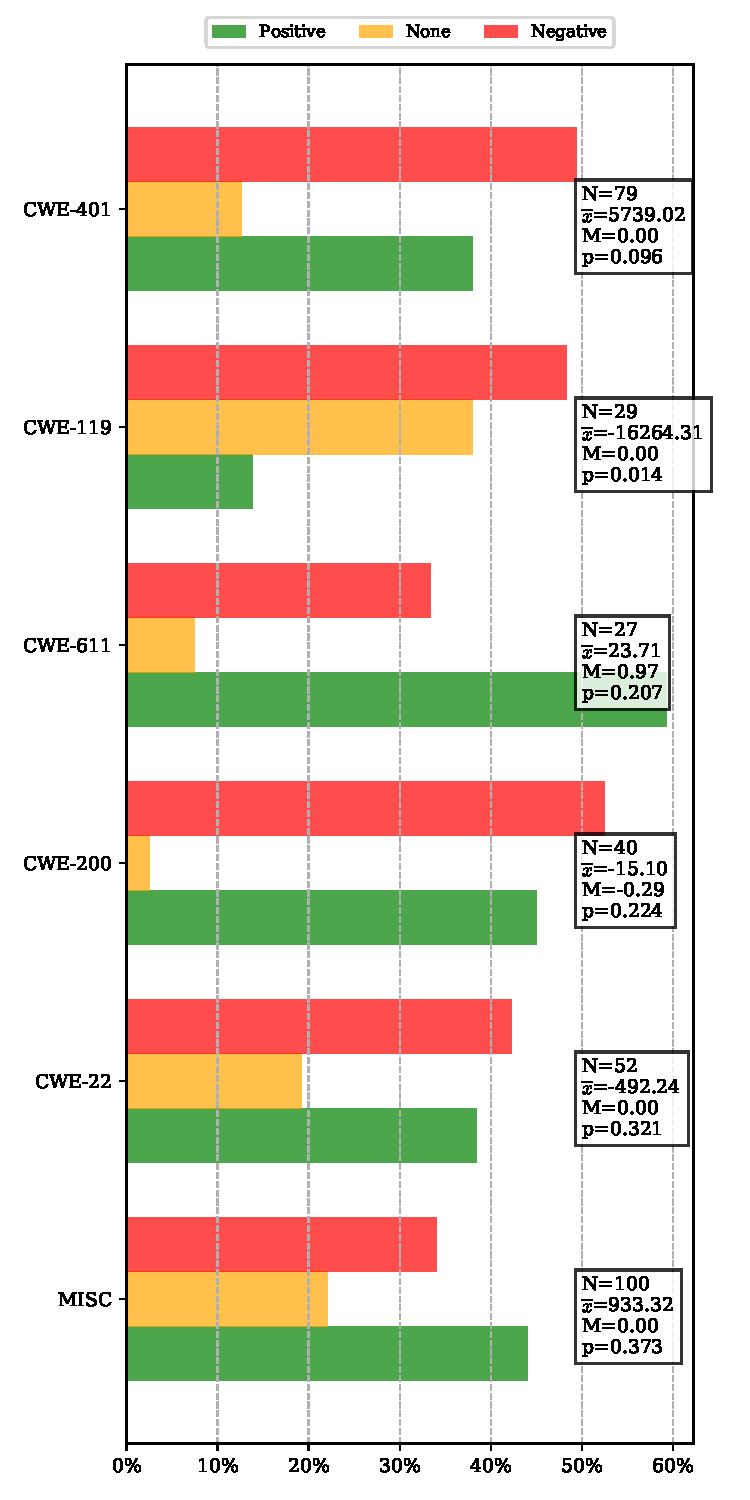
\includegraphics[scale=0.4]{figures/main_per_cwe_spec_664.pdf}}
	\label{fig:pat}
\end{figure*}

\emph{Weakness}, according to Common Weakness Enumeration (CWE) glossary, 
is a type of mistake that, in proper conditions, could contribute to the 
introduction of vulnerabilities within that product. This enumeration
system was used to classify the vulnerabilities included in our study.
Figure~\ref{fig:pat} shows three different charts: \emph{(a)} shows
the impact of all patches grouped using the first-level weaknesses from
the \emph{Research Concepts} list on CWE; and, the remaining charts
show two of those first-level weaknesses more in depth reporting the impact 
on maintainability of their sub-weaknesses (\emph{(b) and (c)}). 

Considering the first-level weaknesses from the \emph{Research Concepts}
list (Figure~\ref{fig:pat}-\emph{a}), we observe that patching vulnerabilities
have negative impact in $5$ weaknesses: Insufficient Control Flow Management 
(CWE-691), Protection Mechanism Failure (CWE-693), Improper Access Control 
(CWE-284), Improper Neutralization (CWE-707) and Improper Control of a Resource 
Through its Lifetime (CWE-664). The CWE-707 ($301$) and CWE-664 ($321$) 
weaknesses integrate a larger amount of cases compared to the remaining 
weaknesses. Thus, we present an analysis of their sub-weaknesses on 
Figure~\ref{fig:pat}-\emph{b} and Figure~\ref{fig:pat}-\emph{c}, respectively. 
Results demonstrate evidence that patching vulnerabilities hinders 
the maintainability of open-source software for $5$ different weaknesses: 
\emph{Improper Input Validation (CWE-20)}, \emph{Information Exposure 
(CWE-200)}, \emph{Improper Restriction of Operations within the Bounds of 
a Memory Buffer (CWE-119)}, \emph{Missing Release of Memory after Effective 
Lifetime (CWE-401)} and \emph{Path Traversal (CWE-22)}. Results also show that 
software maintainability is less negatively impacted when patching 
\emph{Improper Restriction of XML External Entity Reference (CWE-611)}.  

\emph{Cross-Site Scripting (CWE-79)} is the weakness that suffers less 
positive/negative impact from security patches, i.e., patching usually 
has no impact on the maintainability of open-source software. This can 
be explained by the fact that patches to this weakness usually are easily 
done by adding an \texttt{escape} function. Patches of \emph{SQL Injection
(CWE-89)} weaknesses equally hinder and improve the software maintainability. 
But overall a very considerable percentage of patches hinder the open-source 
software maintainability - between $30\%$ and $60\%$. 

Statistical significance was only found to the CWE-119 weakness (p-value = 
$0.041$). However, results obtained to the other weaknesses should not be 
disregarded because they offer an interesting view on how the maintainability 
is impacted per weakness which can provide insights to developers/researchers
on the weaknesses that need more attention.

\textit{\textbf{RQ3: What is the impact of security patches versus regular 
patches on the maintainability of open-source software?}}

The impact of security and baseline changes in the maintainability of
open-source software is presented in Figure~\ref{fig:secvsreg}.  
We have seen, previously, a deterioration on software maintainability 
when patching vulnerabilities: $41.28\%$ ($412$) suffered a 
negative impact, $20.64\%$ ($206$) remained the same and $38.08\%$ 
($380$) increased the software maintainability. For regular changes, 
we observe that the maintainability decreases in $27.05\%$ ($270$) 
and increases in $30.26\%$ ($302$) of the cases. But in contrast to 
security patches, the maintainability of regular changes remains the 
same in $42.69\%$ ($426$) of the cases and performing regular
changes has a more positive impact than negative on the software 
maintainbility. 

Results show that regular changes typically have no impact on the 
software maintainability which contradicts previous research.
However, we manually inspected a considerable amount of cases from
the regular changes distribution where this happens and found that 
identifying regular commits as similar in size as the security-related 
commit is limiting the type of regular commits (e.g, input 
refactorings, variables or functions, type conversion, etc).  
One example is the regular commit\footnote{Regular change: 
\url{https://github.com/AFNetworking/AFNetworking/compare/9cde4e45845486bdb46ad32
2448f93df3b8479bf...3486a008a1fd1348d0f2fe748a5e23933d94647a}} generated 
by our methodology and using as reference the following security commit
\footnote{Security change: 
\url{https://github.com/AFNetworking/AFNetworking/compare/49186d9a3032dc02da1d0cc
445cbf69b0cfb001b...2b2558a90e7bfb2ef5169b1ca21b91851e5a5b7d}}. From a
overflow vulnerability patch, our methodology chose a similiar
type of change. We strongly believe that this phenomenon lead
that increased significantly the number of cases with no impact
on the software maintainability.

The resulting p-value of the Paired Wilcoxon signed-rank test is $0.331$, i.e., 
conclusions regarding the regular changes are not statistically significant. 
Yet, it is important to note that \emph{patching security vulnerabilities seem 
to have a more negative impact on the maintainability of open-source software 
sthan performing regular changes}.

\begin{figure}[h]	
 	\centering 	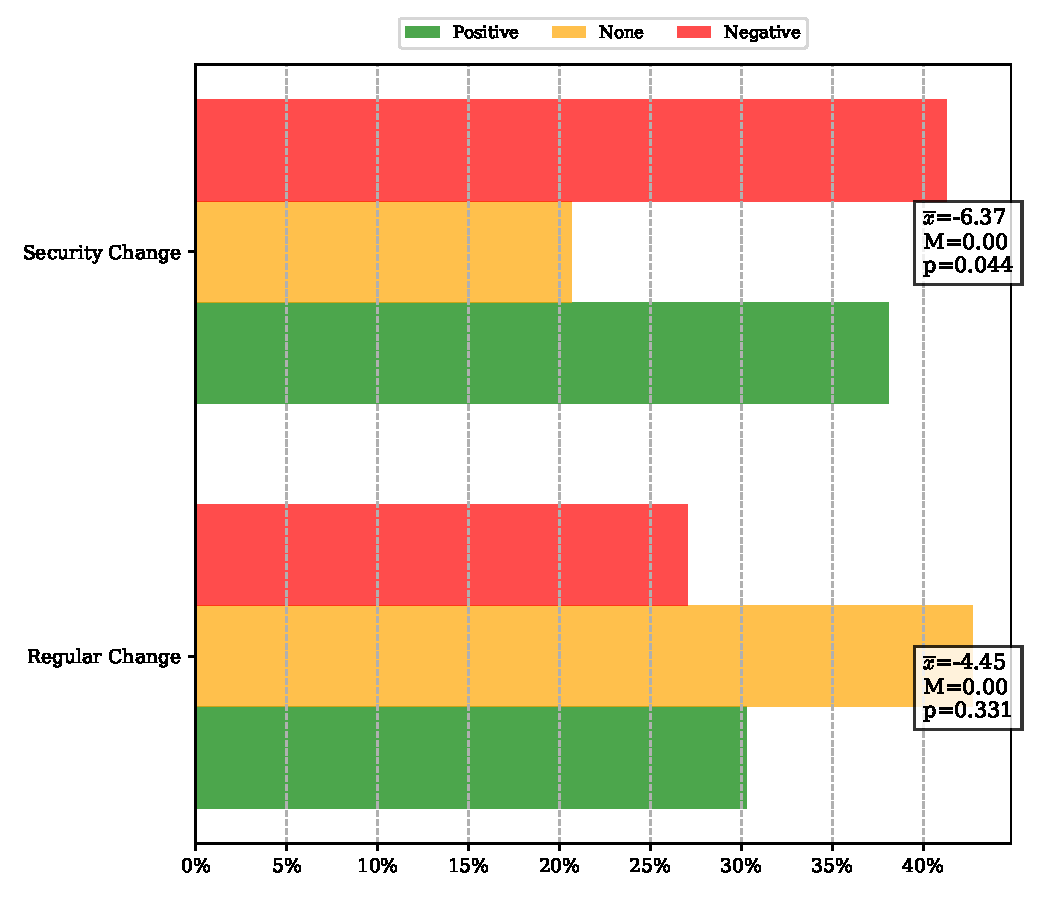
\includegraphics[width=0.4\textwidth]{figures/main_comparison.pdf}
 	\caption{Maintainability difference for security and baseline patches.}
	\label{fig:secvsreg}
\end{figure}

% \section{Discussion}\label{sec:discussion}
%
% In this section, we discuss the results and answer the proposed research
% questions.
%
% \textit{\textbf{RQ1: What is the impact of security patches on the
% maintainability of open-source software?}}
% \textit{Patching vulnerabilities may harm the maintainability of open-source
% software.}
%
% The guideline analysis suggests that all guidelines are affected by security patches. Being the
% \emph{Write Short Units of Code}, \emph{Write Simple Units of Code} and \emph{Separate Concerns in Modules} the guidelines with higher negative impact on the maintainability ($>30\%$ of cases). \emph{Keep Architecture Components Balanced} is the guideline with lower negative impact on
% the maintainability (approx. $10\%$). This might imply that developers should give different
% levels of attention to the guidelines when patching vulnerabilities.
% %
% As expected, vulnerabilities with higher severity are more likely to impact negatively
% the maintainability of software. This suggests that high/medium severity vulnerabilities may
% need more attention than low severity when patching vulnerabilities.
% %
% We would expect that the negative impact of programming languages on
% maintainability to be more severe, as arguably poor design of programming
% languages and lack of using the best practices lead to more buggy and vulnerable
% code~\cite{Ray:2017:LSP:3144574.3126905, 2019arXiv190110220B}. However,
% Figure~\ref{fig:lang_main} shows that only \emph{C/C++} and \emph{Python} have a negative impact approximate to $50\%$ on software maintainability. We suspect that these values are
% the result of projects contributions policies. Nine of the top-10 of dataset projects
% with more contributors have restrict contribution policies regarding code
% standards. Some examples are the \texttt{laravel/framework},
% \texttt{php/php-src}, \texttt{openssl/openssl} and \texttt{cakephp/cakephp}. For
% instance, \texttt{laravel/framework} requires the \texttt{PSR-2
% Standard}\footnote{PSR-2 Standard available at
% \url{https://www.php-fig.org/psr/psr-2/} (Accessed on \today{})} that is a coding style guide for \texttt{PHP}.
%
% \subsubsection*{\textit{\textbf{RQ2} \textbf{Which patterns of security patches are more likely to
% affect open-source software maintainability?}}}
%
%
% \textit{Path Traversal (CWE-22), Information Exposure (CWE-200), Resource Management Errors (CWE-399) are more likely to affect
% open-source software maintainability.}
%
% Overall, the results obtained for the maintainability per CWE are no statistical significance
% The impact of a patch depends on its complexity, i.e., if the patchs
% adds complexity to the code base it is probably affecting the software
% maintainability. One evidence of that is the fact of \emph{Cross-Site Scripting} (CWE-79)
% patches endure more
% cases without any impact in the maintainability. Typically, these types of
% vulnerabilities do not need extra lines to be fixed, as shown in
% Listing~\ref{lst:fix}. Whereas, \emph{Resource Management Errors} (CWE-399) and vulnerabilities
% such as the one presented in Section~\ref{sec:motivation} responsible by Denial-of-Service
% attacks are more difficult to fix (several code lines deleted and added).
% Another example is the Apple authentication flaw discovered in $2017$
% (CVE-$2017$-$13872$)\footnote{CVE-$2017$-$13872$ details available at
% \url{https://support.apple.com/en-us/HT208315} (Accessed on \today{})}, where any user
% could log in as root with an empty password. Patrick Wardle examined the cause
% of the issue\footnote{\emph{Why $<$blank$>$ Gets You Root} available at
% \url{https://objective-see.com/blog/blog\_0x24.html} (Accessed on \today{})} and
% concluded that the flaw was due to the introduction of high cyclomatic complexity
% in a method used to verify the password. In sum, \emph{Cross-Site Scripting} (CWE-79) should take part of the
% developers' preoccupations along with the other patterns that explicitly hinder
% maintainability because despite their low complexity these are patterns that
% still produce a considerable negative impact on the maintainability. Real
% efforts have been made in creating and incorporating coding standards and best
% practices in software production. However, security is still far from perfection
% and fixing vulnerabilities might hinder software maintainability. Thus, it is
% not only important to provide tool support to developers to help them apply these
% patterns without harming software maintainability, but also to create and redesign
% programming languages to facilitate developers improving software maintainability.
%
% We measured the effect sizes between both distribution -- before and after
% patches --- per language and security patterns using the Common Language Effect
% Size~\cite{cliff:1993} method. Effect sizes are of a low-medium level.
% Thus, considering the $0$ median and the low effect sizes, it is reasonable
% to affirm that there is a significant effect but it might only be
% recognized after a thoughtful data analysis.
%
%
% \subsubsection*{\textit{\textbf{RQ3} \textbf{What is the impact of security patches versus regular changes
% on the maintainability of open-source software?}}}
% \textit{Patching security vulnerabilities has a larger negative and positive impact
% than when fixing regular commits.}
%
% We found that $41.76\%$ of the security patches have a negative impact on the
% maintainability of open-source software (cf. Figure~\ref{fig:secvsreg}). While $21.04\%$ of regular commits have a negative impact on the maintainability. This raises
% a new trade-off when developers need to patch vulnerabilities on their projects
% because they might be affecting the software maintainability or even introducing
% new vulnerabilities. This study exhibits evidence that developers may have to
% reduce maintainability for the sake of security. We understand that developers
% should be able to produce secure code without affecting the maintainability of
% their projects. But there are still some concerns that need to be addressed:
% \begin{itemize}
% 	\item \textbf{Documentation} of software must provide developers with the
% 	best practices to implement secure and maintainable software. Unmaintainable
% 	code is difficult to test, analyze and re-use.
%
% 	\item\textbf{Programming Languages} should provide new design patterns to
% 	easily implement security patterns without endangering maintainability.
% 	Ultimately, new programming languages, both secure and maintainable by design,
% 	may be designed to help developers be highly productive when writing and
% 	maintaining  secure applications. One example is the need for designing new
% 	authorization mechanisms since these are one of the most complex security
% 	features to implement.
%
% 	\item \textbf{Software Developers} lack the knowledge to create secure and
% 	maintainable code. Mainly because academic curricula are not yet prepared
% 	to properly educate them. Universities should do their part on making
% 	this possible. Online services such as BCH have also a great potential to help
% 	developers to be more aware of the maintainability issues introduced by their
% 	changes. Thus, developers can put more work into improving their code maintainability
% 	and avoid common issues such as code duplication.
%
% \end{itemize}



\section{Threats to Validity}\label{sec:threats}
%
The following section presents the potential threats to the validity of this
study.
%
\\\textit{\textbf{Construct:}} The maintainability formula was inferred based 
on the BCH's reports. The high amount of different projects and backgrounds 
may require other maintainability standards. However, BCH does use a 
representative benchmark of closed and open-source software projects to compute 
the thresholds for each maintainability guideline~\cite{Visser:2016:OREILLY, Baggen2012}.
%
\\\textit{\textbf{Internal:}} The security patches dataset provided by previous
work~\cite{Reis:2017:IJSSE} was collected based on the messages of GitHub
commits produced by project developers to classify the changes performed by them
to fix security flaws. This approach discards security patches that were
not explicit in commits messages. Pontas et. al\cite{10.1109/MSR.2019.00064} dataset
has patches that were manually mined in software repositories. Being a manual technique,
the search might led to
wrong associations between vulnerabilities and code snippets.
Baseline commits are retrieved randomly by selecting one commit from the same
project of a given security patch. This approach softens the differences
that may result from the characteristics of each project. However,
maintainability may still be affected by the developers' experience, coding
style and software contribution policies which is not evaluated in this study.
Furthermore, this evaluation considers that $998$ regular commits are enough to
alleviate random irregularities in the maintainability differences of the
baseline.
%
\\\textit{\textbf{External:}} We use a dataset that only comprises patches of open-source software.
However, the methodology requires to access data that is not publicly available.
Thus, our findings may not extend to non-open source software. Different programming 
languages may require different coding practices to address software safety. The 
dataset comprises more commits in Java, i.e., the dataset may not be representative 
of the population regarding programming languages. Our approach does not consider 
security patches in any other languages but English.

\section{Related Work}\label{sec:rw}

Many studies have investigated the relationship between refactorings and
software quality. Previous work focused on object-oriented metrics has evaluated the
impact of refactorings and exhibited proof that quantifying effectively the
impact of refactorings on maintainability may help to choose the appropriate
refactoring type~\cite{1167822}. In contrast to this work, Hegedus et
al.~\cite{HEGEDUS2018313} did not select particular metrics to assess the effect
of refactorings. Instead, statistical tests were used to find the metrics that
have the potential to change significantly after refactorings. The differences
of maintainability between groups of refactored elements and non-refactored were
analyzed. In addition, the authors concluded that the source code elements
subjected to refactorings had significantly lower maintainability than the
elements not affected. Studying the evolution of maintainability issues during
the development of Android apps, Malavolta et al. ($2018$)~\cite{8530041}
discovered that maintainability decreases over time. Palomba et al.
($2018$)~\cite{Palomba:2018:DIM:3231288.3231337} exhibits proof that code smells
should be carefully monitored by programmers since there is a high correlation
between maintainability aspects and proneness to changes and faults. In 2019, Luis et 
al.~\cite{cruz2019energyoriented} proposed a formula to calculate maintainability 
based on the BCH's guidelines and measured the impact of energy-oriented fixes 
on the maintainability of software.
The present work uses the same model (BCH) and focuses solely on evaluating 
the impact of patching vulnerabilities on software maintainability.

Researchers investigated the relationship between design patterns and software
maintainability~\cite{10.1007/978-3-642-35267-6-18}. $300$ revisions of
\texttt{JHotDraw} were analyzed to conclude that every introduced pattern
instance improved software maintainability. However, other studies show that the
use of design patterns may introduce maintainability issues into
software~\cite{4493325}. Yskout et. al were not able to detect if the usage of 
design patterns has a positive impact, but concludes that developers prefer to 
work with the support of security patterns~\cite{8077802}. The present work 
studies how security patterns influence maintainability for open-source software.

There are studies that investigated the impact of programming languages on software
quality~\cite{Ray:2014:LSS:2635868.2635922,Ray:2017:LSP:3144574.3126905}. The first
study shows that some programming languages are more buggy-prone than others. However,
the authors of the second study were not able to reproduce it, not obtaining any
evidence about the impact of language design. Both have used the number of
defects as an indicator of software quality. In addition,
Berger et al. ($2019$)~\cite{2019arXiv190110220B} tried to reproduce~\cite{Ray:2014:LSS:2635868.2635922,
Ray:2017:LSP:3144574.3126905} and identified flaws that throw into distrust the 
previously demonstrated correlation between programming language and software 
defects. Our work studies how security refactorings affect software quality based 
on the code maintainability analysis and provides evidence that programming languages 
have an impact on maintainability.

\section{Conclusion and Future Work}\label{sec:conclusions}

This work presents an empirical study on the impact of $998$ security
patches on the maintainability of $262$ open-source projects. We leveraged
Better Code Hub reports to calculate maintainability based on a model proposed in previous work~\cite{Olivari:2018, cruz2019energyoriented}. Security patches 
significantly affect the software maintainability of open-source software, i.e., 
developers hinder maintainability when patching vulnerabilities. We found this evidence in
$41.28\%$ of the studied cases. Regarding regular commits, it seems that overall
maintainability stays the same ($42.69\%$). However, there is still a 
considerable amount of cases that harm maintainability ($27.05\%$).

This study also shows evidence that there are security patterns that need more
attention than others. \emph{Improper Input Validation} (CWE-20), \emph{Information 
Exposure} (CWE-200), \emph{Improper Restriction of Operations within the Bounds of a 
Memory Buffer} (CWE-119), \emph{Missing Release of Memory after Effective Lifetime} 
(CWE-401) and \emph{Path Traversal} (CWE-22) endure maintainability
in $41.9\%$, $52.5\%$, $42.9\%$, $49.4\%$, and $41.7\%$, respectively. Therefore, 
we draw attention for the need of better documentation explaining how to use best practices to
produce secure and maintainable code; new and better programming languages; new
academic curricula in the fields of security and software quality; and, tools
such as BCH to help developers predict the effect of their patches.

As future work, this study may be extended in several directions: 
investigate what are the most frequent vulnerabilities in each programming
language; investigate how patches impact maintainability for each
vulnerability and programming language;
study if there is any correlation between code maintainability and
the popularity of a software project; expand our methodology with other
software quality properties; validate these findings with closed or private
software; and, expand this analysis to other quality standards.


%
% \section*{Acknowledgment}\label{sec:ack}
%
% \noindent
% We thank the Software Improvement Group (SIG) team for all the support and
% help in validating the methodology.
% %ack pedro adao when accepted.
% \pagebreak
\balance

{
  \bibliographystyle{unsrt}
  \bibliography{icsme20}
}

\end{document}